\documentclass[a4paper,pdflatex,sn-mathphys-num]{sn-jnl}
% Compact preprint layout for arXiv.  The journal class otherwise reserves
% unusually wide asymmetric margins intended for the production workflow.
\geometry{
  a4paper,
  left=18mm,
  right=18mm,
  top=18mm,
  bottom=20mm,
  bindingoffset=0pt
}
% Data figures are compiled from editable PGF/TikZ sources as vector PDFs;
% the MAC sketch is drawn directly in TikZ below.
\usepackage{graphicx}
\usepackage{amsmath,amsthm,amsfonts,amssymb}
\theoremstyle{thmstyleone}
\newtheorem{lemma}{Lemma}
\newtheorem{proposition}{Proposition}
\newtheorem{theorem}{Theorem}
\usepackage{xurl}
\urlstyle{same}
% Keep DOI domains and identifier segments intact; break at separators.
\newcommand{\doiurl}[1]{%
  \begingroup
  \def\UrlBreaks{\do\/\do\-\do\_\do\;\do\:\do\)}%
  \url{https://doi.org/#1}%
  \endgroup
}
\usepackage{pgfplots}
\usepgfplotslibrary{groupplots}
\pgfplotsset{compat=1.18}
% Use compact superscripts for powers of ten on logarithmic axes.
\pgfplotsset{log number format basis/.code 2 args={$#1^{\scriptscriptstyle\pgfmathprintnumber{#2}}$}}
% Put unboxed plot legends below their axes. Group plots may replace these
% defaults with one shared legend below the complete panel group.
\pgfplotsset{legend style={
  draw=none,
  fill=white,
  fill opacity=1,
  text opacity=1,
  inner sep=2pt,
  at={(0.5,-0.24)},
  anchor=north,
  legend columns=-1
}}
\pgfplotscreateplotcyclelist{journalcycle}{
  {blue!75!black,solid,thick,mark=*},
  {orange!90!black,solid,thick,mark=square*},
  {green!60!black,solid,thick,mark=triangle*},
  {red!75!black,solid,thick,mark=diamond*},
  {black,dashed,thick,mark=x}
}
\pgfplotsset{journalaxis/.style={
  width=0.42\textwidth,
  height=0.30\textwidth,
  cycle list name=journalcycle,
  grid=major,
  grid style={gray!25},
  axis line style={black},
  tick align=outside,
  major tick length=2pt,
  minor tick length=1pt,
  tick label style={font=\sffamily\small},
  label style={font=\sffamily\small},
  title style={font=\sffamily\small},
  legend style={font=\sffamily\small}
}}
\usepackage{float}
\usepackage[hypcap=false,font=footnotesize,labelfont=bf,labelsep=space]{caption}
\usepackage{flafter}
\usepackage{placeins}
% Allow flexible float placement to avoid sparse pages.
\setcounter{topnumber}{3}
\setcounter{bottomnumber}{2}
\setcounter{totalnumber}{5}
\renewcommand{\topfraction}{0.9}
\renewcommand{\bottomfraction}{0.8}
\renewcommand{\textfraction}{0.08}
\renewcommand{\floatpagefraction}{0.65}
\usepackage{booktabs}
\usepackage{xcolor}


% 绘图核心包（基础图形、流程、示意图依赖）
\usepackage{bm}                           % 粗体向量 \bm{v}
\usepackage{mathtools}                    % AMS math 的增强版


\usepackage{tikz}
\usetikzlibrary{%
  arrows,          % 箭头
  calc,            % 坐标计算
  3d,              % 3D 坐标
  shapes,          % 图形形状
  positioning,     % 相对位置
  backgrounds,     % 背景层
  decorations.pathreplacing, % 花括号装饰线
  patterns,        % 填充图案
  intersections,   % 线段交点
  matrix           % 矩阵布局
}


% 数据可视化包（曲线、柱状、3D、极坐标图依赖）

\usepackage{pgfplots}

% 固定PGFPlots版本兼容性（避免不同版本语法冲突，建议使用1.18及以上）

\pgfplotsset{compat=1.18}

% 加载TikZ扩展库（图案、箭头、几何形状、阴影、背景、定位）

\usetikzlibrary{patterns, arrows.meta, shapes.geometric, shadows, backgrounds, positioning}
% 核心配色：RGB值已转换为LaTeX支持的0-1范围（避免颜色显示异常）

\definecolor{nature-blue}{RGB}{0, 114, 178}    % 主蓝色（实验组、关键元素）

\definecolor{nature-red}{RGB}{213, 94, 0}      % 橙红色（对照组、警示元素）

\definecolor{nature-green}{RGB}{0, 158, 115}   % 绿色（处理组、正向元素）

\definecolor{nature-yellow}{RGB}{240, 228, 66} % 黄色（辅助元素、高亮）

\definecolor{nature-purple}{RGB}{204, 121, 167}% 紫色（特殊流程、次要元素）

\definecolor{nature-gray}{RGB}{86, 86, 86}     % 深灰色（网格、边框、文字）

% 淡色系列（流程图背景、辅助区域）

\definecolor{light-blue}{RGB}{230, 240, 250}   % 淡蓝色

\definecolor{light-red}{RGB}{255, 235, 220}    % 淡橙色

\definecolor{light-green}{RGB}{220, 245, 235}  % 淡绿色

% Standard pseudocode; the unmodified package is bundled with the source.
\usepackage[ruled,lined,linesnumbered,longend]{algorithm2e}
\SetAlFnt{\small}
\SetAlCapFnt{\small}
\SetAlCapNameFnt{\small}
\SetAlgoNlRelativeSize{-1}
\DontPrintSemicolon
\SetKwInOut{Input}{Input}
\SetKwInOut{Output}{Output}
\newcommand{\printbibliography}{%
  \bibliography{ref}%
}
\providecommand{\bibcommenthead}{}

% Avoid stretching spaces between paragraphs to equalize page heights.
\raggedbottom
\begin{document}
\title[Treecode Hartree evaluation on locally refined meshes]{A Treecode Algorithm for Hartree Potential Evaluation on Locally Refined Meshes}

\author[1]{\fnm{Huan} \sur{Xiao}}\email{yc37985@um.edu.mo}
\author[2]{\fnm{Zixuan} \sur{Cui}}
\author*[1]{\fnm{Guanghui} \sur{Hu}}\email{garyhu@um.edu.mo}

\affil[1]{\orgdiv{State Key Laboratory of Internet of Things for Smart City
  and Department of Mathematics}, \orgname{University of Macau},
  \orgaddress{\city{Macau}, \country{China}}}
\affil[2]{\orgname{The Chinese University of Hong Kong, Shenzhen},
  \orgaddress{\country{China}}}

\abstract{

Attosecond physics relies on time-dependent electronic structure calculations,
which require the long-range Coulomb (Hartree) potential at every time step.
This repeated evaluation is a major computational cost in real-space
formulations. Adaptive finite element meshes reduce discretization cost through local
refinement, while the Hartree potential still requires efficient free-space
evaluation on the resulting nonuniform mesh. We therefore develop a treecode for Hartree potential evaluation on
locally refined meshes of the type generated by Kohn--Sham DFT calculations. Under the bounded-work assumptions stated below and for fixed evaluation parameters, the method has $O(N\log N)$ work, compared with $O(N^2)$ for direct summation. Its hierarchical neighborhood search builds candidate source regions from vertex incidence and parent--child links in the existing refinement tree; recursive materialization and MAC classification then produce disjoint near- and far-field lists. Numerical experiments with prescribed single-center and multicenter densities demonstrate the accuracy and efficiency of the method. At fixed evaluation parameters and comparable leaf counts, adaptive refinement reduces the sampled error by factors of 16.2 and 9.5 on the two finer mesh pairs, while reducing total runtime by 8.5\% and 12.0\%, respectively. Potential evaluation achieves a 57.93-fold speedup on 64 CPU threads.}

\keywords{Hartree potential, locally refined tetrahedral meshes, treecode,
Kohn--Sham density functional theory, fast summation method}

\maketitle

\section{Introduction}
Electronic structure calculations underpin much of nanoscience
\cite{Ogut2003} and, through real-time propagation, of attosecond physics,
where electronic states are followed on their natural timescale
\cite{LopataGovind2011}. Many of these systems are finite or only partially
periodic and geometrically irregular, so a free-space Coulomb description and a
spatially nonuniform resolution are both natural.
The ground state is governed by the many-electron Schr\"odinger equation, whose
direct solution is prohibitive because the wavefunction depends on all electronic
coordinates. Density functional theory (DFT) instead takes the electron density
as the basic variable \cite{Hohenberg1964,Parr1989,Martin2004,Jones2015}, and the
Kohn--Sham formulation \cite{Kohn1965} expresses it through single-particle
orbitals satisfying, in atomic units,
\begin{equation}
\label{eq:kohn_sham}
\left[
-\frac{1}{2}\nabla^2
+V_{\mathrm{ext}}
+V_H[\rho]
+V_{\mathrm{xc}}[\rho]
\right]\psi_i
=\varepsilon_i\psi_i,
\end{equation}
Here, \(\mathbf r\) denotes position, while \(\psi_i\), \(\varepsilon_i\), and \(f_i\) denote the \(i\)th orbital, its eigenvalue, and its occupation number. With \(N_{\mathrm{orb}}\) occupied orbitals, the electron density is
\begin{equation}
\label{eq:electron_density}
\rho(\mathbf r)=\sum_{i=1}^{N_{\mathrm{orb}}}f_i|\psi_i(\mathbf r)|^2,
\qquad \sum_{i=1}^{N_{\mathrm{orb}}}f_i=N_e.
\end{equation}
The effective potential consists of the external potential \(V_{\mathrm{ext}}\), the exchange–correlation potential \(V_{\mathrm{xc}}\), and the Hartree potential \(V_H\), defined as
\begin{equation}
\label{eq:hartree}
V_H(\mathbf r)
=\int_{\mathbb R^3}
\frac{\rho(\mathbf r')}{|\mathbf r-\mathbf r'|}
\,d\mathbf r'.
\end{equation}
The Hartree term is nonlocal: it couples each target to the whole source domain
and must be recomputed whenever the density changes, at every self-consistent
field (SCF) iteration and at every time step of a real-time propagation. Direct
summation over $N$ source elements at a comparable number of targets costs
$O(N^2)$ per evaluation, so this term dominates the cost as the system or the
number of steps grows. Since these repeated evaluations often share a fixed or
only occasionally updated mesh, an evaluator whose geometric data structures can
be built once and reused across density updates is particularly attractive,
provided it remains accurate on a locally refined mesh.
Adaptive finite element methods reduce the discretization cost by refining only
where needed \cite{BaoHuLiu2012,HuXieXu2018,YangShenHu2021,Hu2026}, with separate
adaptive meshes even used for the Kohn--Sham and Poisson equations
\cite{Kuang2024}. The Hartree term, however, must still be evaluated on the
resulting mesh. Solving the Poisson equation $-\nabla^2 V_H=4\pi\rho$ by finite
elements requires boundary data that approximate the free-space solution
\cite{BaoHuLiu2012,Kuang2024}, whereas the integral formulation
in~\eqref{eq:hartree} evaluates the Coulomb interaction directly and keeps the
source-truncation error explicit. Becke's fuzzy-cell partition organizes
molecular quadrature into atom-centered contributions \cite{Becke1988Multicenter}
but does not by itself accelerate the long-range part. Here we retain the
adaptive tetrahedral mesh and evaluate the Hartree integral by fast summation.

Fast summation accelerates such convolutions either on structured grids, using
FFT-based methods or particle-mesh Ewald \cite{Genovese2006,Darden1993}, or by
hierarchically grouping sources, as in the fast multipole method
\cite{Greengard1987,Yokota2013,JiangGreengard2025} and in treecodes, which
evaluate source expansions at individual targets \cite{Appel1985,Barnes1986}.
Grid-based approaches require an auxiliary regular grid on an adaptive
tetrahedral mesh, whereas a treecode can exploit the tetrahedral refinement
hierarchy directly and keeps targets independent. TAGI applies a barycentric
Lagrange treecode to discrete sums over Chebyshev quadrature points on
a-priori refined cuboid grids \cite{TAGI2020}; in the present setting the
sources are integrals over tetrahedral elements and the hierarchy is the
refinement tree of an existing locally refined mesh. Cui et al. built geometric
near- and far-field patches for a mesh-based Poisson treecode \cite{Cui}, and
Cui and Yang adapted expansion orders to local error requirements
\cite{CuiYang2025}; their geometric construction motivates our extension to
locally refined meshes.

On a locally refined mesh, active elements differ in size and refinement level,
so two problems must be solved: the sources must be covered exactly once, and
the separation that justifies a multipole expansion must be tested explicitly.
Within AFEPack \cite{AFEPack}, our hierarchical neighborhood layer (HNL)
construction uses level-indexed vertex incidence and parent--child links to
collect candidate regions through successively coarser levels, without scanning
the whole mesh at each level, and a recursive traversal converts them into a
disjoint cover. A multipole acceptance criterion (MAC) \cite{Barnes1986,Cui}
then accepts sufficiently separated clusters for multipole evaluation,
subdivides rejected clusters, and retains rejected leaves for direct
integration. The resulting lists depend only on the geometry and the acceptance criterion.

The novelty of the present work lies in the mesh on which the treecode
operates. To the best of our knowledge, this is the first Hartree treecode to be
constructed, analyzed, and validated on the refinement hierarchy of an
h-adaptive tetrahedral finite element mesh. This statement concerns the
algorithm and its validation rather than the data structure: earlier
hierarchy-geometry-tree treecodes can represent such non-full trees but assume a
uniform refinement level and list adaptive mesh refinement as future work
\cite{Cui,CuiYang2025,CuiYangHu2025}, and h-adaptive Kohn--Sham calculations use the same tree
for mesh management while solving a Poisson equation for the Hartree potential
\cite{Kuang2024}. Concretely, we (i) build the source search directly on the
existing refinement tree, without a separate spatial tree; (ii) give a recursive
materialization yielding a complete, nonoverlapping source cover that MAC
classification preserves; and (iii) separate geometry-dependent interaction
lists from density-dependent moments, supported by complexity and error
analyses and a multithreaded implementation. These advantages are structural
rather than comparative: no auxiliary uniform grid or separate spatial tree is
required, the free-space Coulomb kernel is retained without a
boundary-condition approximation, and the lists are reusable with independent
targets. The contribution is that fast free-space Hartree evaluation
becomes available directly on a locally refined finite element mesh, using a
hierarchy that the adaptive calculation has already built.

Numerical experiments with prescribed single-center and multicenter densities demonstrate the accuracy and efficiency of the proposed method. In the fixed-parameter adaptive--uniform comparison, adaptive refinement gives 9.5 times smaller sampled error on the finest pair with 2.0\% fewer leaf elements and 12.0\% less total runtime. Potential evaluation achieves a 57.93-fold speedup on 64 CPU threads.

The remainder of this paper is organized as follows. Section~\ref{sec:adaptive_meshes_treecodes} introduces adaptive meshes and treecode evaluation. Section~\ref{sec:proposed_method} presents the HNL–MAC algorithm and analyzes its computational cost and error. Section~\ref{sec:numerical_experiments} assesses accuracy, efficiency, and parallel scalability using prescribed densities; coupling to a complete SCF solver remains future work. Section~\ref{sec:conclusions} discusses the results and remaining challenges. Supporting details are provided in the Appendix.

\section{Adaptive Meshes and Treecodes}
\label{sec:adaptive_meshes_treecodes}
\subsection{Adaptive Meshes for Kohn--Sham Calculations}
\label{subsec:adaptive_mesh}

Kohn--Sham orbitals typically vary rapidly near nuclei and more smoothly farther away. Adaptive finite element methods use indicators derived from the computed orbitals to guide local refinement. Following Bao, Hu, and Liu \cite{BaoHuLiu2012}, we form an element indicator from the orbital gradients as
\begin{equation}
\eta_{K,i}=\left(\int_K|\nabla\psi_i|^2\,d\mathbf x\right)^{1/2},
\qquad
\eta_K=\sum_i s_i\,\widehat{\eta}_{K,i},
\label{eq:ks_orbital_indicator}
\end{equation}
where \(\widehat{\eta}_{K,i}\) denotes the normalized indicator for orbital \(i\), and the positive weights \(s_i\) balance the contributions of different orbitals. Elements with large indicators are refined, whereas regions with sufficiently small indicators may be coarsened, subject to mesh compatibility constraints. The resulting mesh is therefore adapted to the computed electronic structure through indicator-driven refinement and coarsening.

The choice of indicator determines which features the mesh resolves. Multilevel correction has been combined with adaptive refinement to reduce the cost of the Kohn--Sham solve \cite{HuXieXu2018}. Residual-based indicators use element residuals and jumps in normal derivatives across element faces; Kuang, Shen, and Hu use such indicators to adapt separate meshes for the Kohn--Sham and Poisson equations \cite{Kuang2024}. The separate meshes allow the orbitals and Hartree potential to be resolved independently. More recently, adaptive real-space grids and Poisson solves have been used in molecular density fitting \cite{Zhu2026}.

Although local refinement reduces the number of elements, each density update still requires Hartree contributions from the entire source domain. We reuse the refinement hierarchy in AFEPack \cite{AFEPack}, including refinement levels, vertex-to-element adjacency, and parent--child links. Active leaf elements partition the domain, and each parent defines a source cluster through its descendant leaves, so no separate spatial tree is needed. The numerical experiments use prescribed densities to assess the Hartree evaluator independently of an SCF solver. A radial refinement indicator serves as a controlled surrogate for the orbital-based indicator in Eq.~\eqref{eq:ks_orbital_indicator}; this isolates the effects of local refinement and treecode parameters from SCF-driven adaptation.

\subsection{Treecodes for Hartree Evaluation}
\label{subsec:treecode}

Treecodes were developed to accelerate $N$-body interactions through hierarchical source grouping; octree-based gravitational simulations are a classical example \cite{Appel1985,Barnes1986}. Each source cluster is represented by multipole moments, allowing its contribution to a sufficiently distant target to be approximated without evaluating every source individually. The MAC decides whether a cluster is sufficiently separated to be accepted \cite{Barnes1986,Dehnen2000}. Rejected clusters are recursively subdivided until a multipole approximation is accepted or a leaf is evaluated directly. At fixed expansion order and MAC parameters, logarithmic tree depth and a bounded number of interactions per target per level yield $O(\log N)$ work per target and $O(N\log N)$ total work for $O(N)$ targets, compared with $O(N^2)$ for direct summation. Treecodes have also been applied to molecular Coulomb interactions \cite{DuanKrasny2001}.

For Hartree evaluation, source contributions are integrals over mesh elements rather than interactions with individual particles. Given a prescribed density \(\rho_h\) on an active leaf mesh \(\mathcal T_h\) of a truncated domain \(\Omega\subset\mathbb R^3\), the potential is
\[
V_H[\rho_h](\mathbf x)
=\int_{\Omega}\frac{\rho_h(\mathbf y)}{|\mathbf x-\mathbf y|}\,d\mathbf y
=\sum_{K\in\mathcal T_h}
\int_K\frac{\rho_h(\mathbf y)}{|\mathbf x-\mathbf y|}\,d\mathbf y.
\]
where $K$ is a source leaf, $\mathbf x$ and $\mathbf y$ are the target and source points, respectively, and $N=|\mathcal T_h|$ is the number of active leaves. Here, $V_H[\rho_h]$ denotes the exact potential generated by $\rho_h$ over the truncated domain. Contributions from leaves in the neighbor list are computed by direct numerical integration, with separate treatment of the kernel singularity. Far-field contributions use Cartesian multipole expansions \cite{BeatsonGreengard1997,Cui}; their moments represent the density over all descendant leaves of each accepted cluster. Thus, accepting a parent cluster preserves the fine-mesh source information through its moments. Under the assumptions detailed in Section~\ref{sec:overall_algorithm}, this evaluation avoids the quadratic scaling of direct summation.

\subsection{Treecode Evaluation on Locally Refined Meshes}
\label{sec:interaction_list_review}

Local refinement reduces the cost of spatial discretization, while treecodes accelerate the evaluation of long-range interactions. Combining these benefits requires a source search that accommodates elements of different sizes and refinement levels. Unlike particle-based methods that construct spatial octrees from particle data, such as Cornerstone \cite{Keller2023}, the present approach uses an existing tetrahedral refinement hierarchy. Two requirements must be satisfied: source regions must be represented without double counting parent--descendant contributions, and each accepted cluster must be sufficiently separated from the target for multipole approximation. Geometric adjacency alone does not guarantee either requirement.

Previous mesh-based Poisson treecodes have used geometric relations to construct near-field and far-field patches \cite{Cui}, with subsequent work adapting expansion orders to local accuracy requirements \cite{CuiYang2025}. Cui, Yang, and Hu also developed a treecode for demagnetizing-field evaluation on general domains, using hierarchy geometry to construct non-neighbor patches and an error-based adaptive multipole order \cite{CuiYangHu2025}. Our problem is Hartree evaluation on locally refined tetrahedral meshes; its source search must follow the mesh refinement hierarchy across elements of different sizes while preventing overlapping parent and descendant representations. These requirements motivate the hierarchical neighborhood search developed here.

We address these requirements in Section~\ref{sec:proposed_method} by separating the source search, which follows the mesh hierarchy, from the source partition, where a recursive materialization yields the cover and the MAC assigns each region to direct integration or multipole evaluation. The main contribution is this hierarchical source search for locally refined meshes, combined with established quadrature and Cartesian multipole expansions.

\section{Treecode with Hierarchical Neighborhood Search}
\label{sec:proposed_method}

For each target leaf, HNL identifies candidate source regions using vertex adjacency and the refinement hierarchy. A recursive traversal turns these candidates into a complete, nonoverlapping cover of the source domain. The MAC then classifies cover regions for direct integration or multipole evaluation while preserving that partition. This section presents these steps, followed by the implementation, computational complexity, and error analysis.

\subsection{Hierarchical Neighborhood Layer Construction}
\label{sec:hnl}

Starting from a target leaf \(K_t\), HNL expands through successively coarser levels. Parent--child links provide access to the refinement hierarchy, and a precomputed vertex-to-element index defines \(\operatorname{star}_j(v)\), the level-\(j\) elements incident on vertex \(v\). At each level, the algorithm queries only vertices of the current layer, adds the sibling families of newly encountered elements as candidates, and moves the search to their parents together with the parents of the current layer. Thus the search follows local mesh connectivity rather than scanning all elements at each level. Figure~\ref{fig:hnl_layerwise_2d} illustrates the resulting layers; their shapes depend on the mesh geometry. HNL selects candidate regions, while the MAC later determines whether each cover region can be approximated by a multipole expansion.

\begin{figure}[!htbp]
\centering
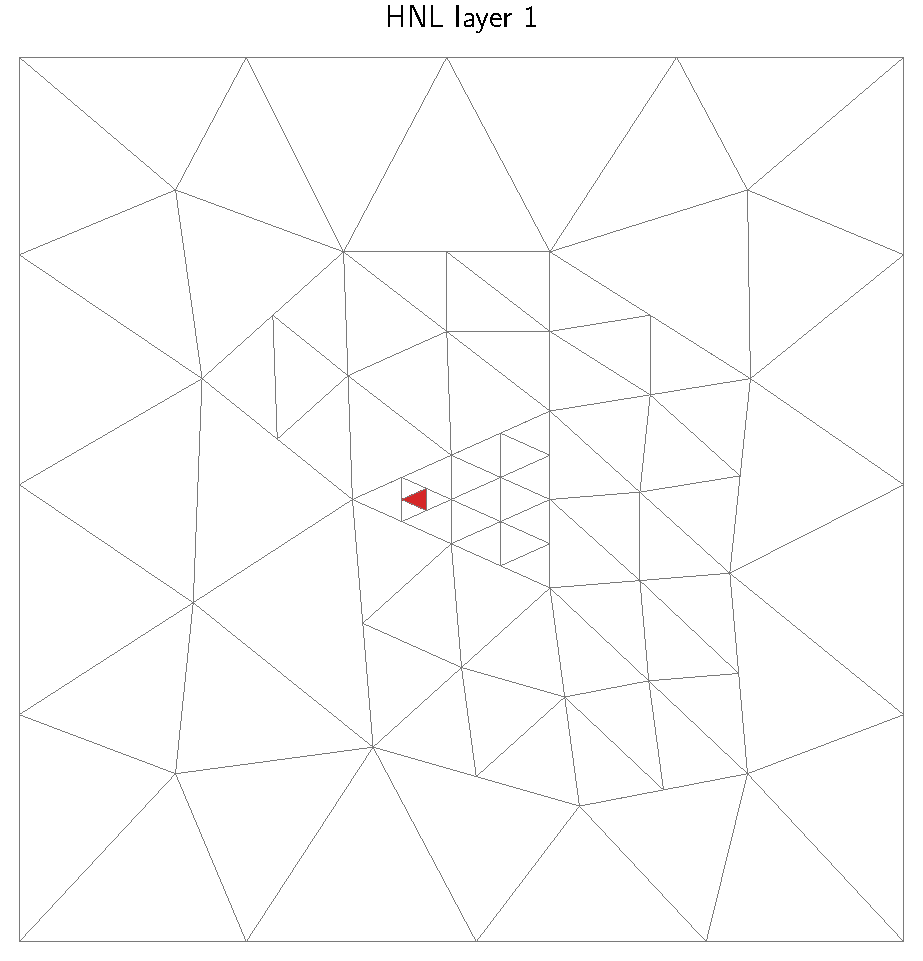
\includegraphics[width=0.31\textwidth]{Fig1a.pdf}\hfill
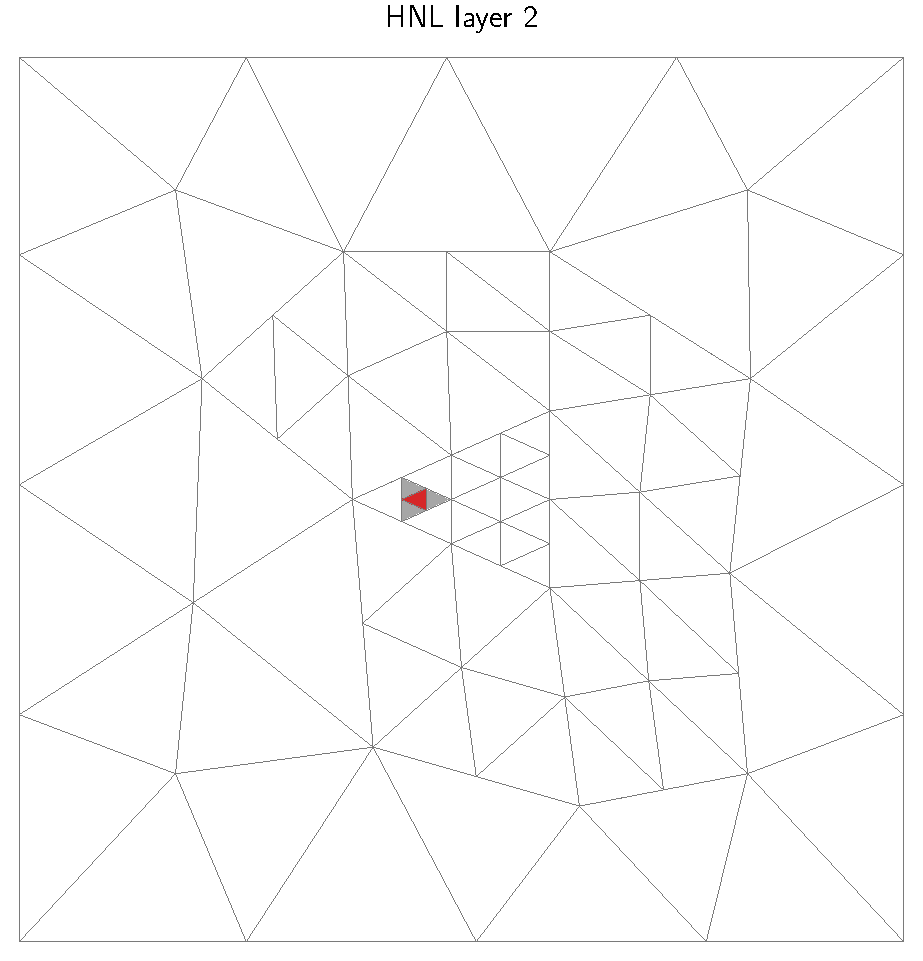
\includegraphics[width=0.31\textwidth]{Fig1b.pdf}\hfill
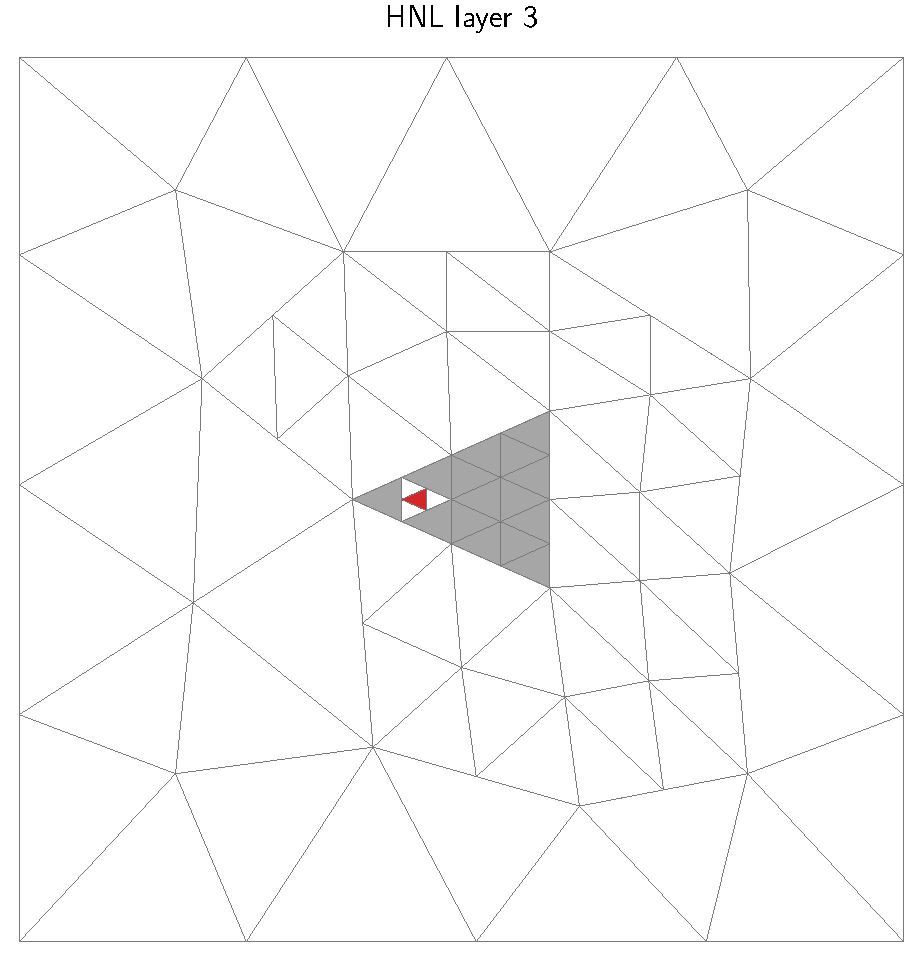
\includegraphics[width=0.31\textwidth]{Fig1c.pdf}\\[-0.35em]
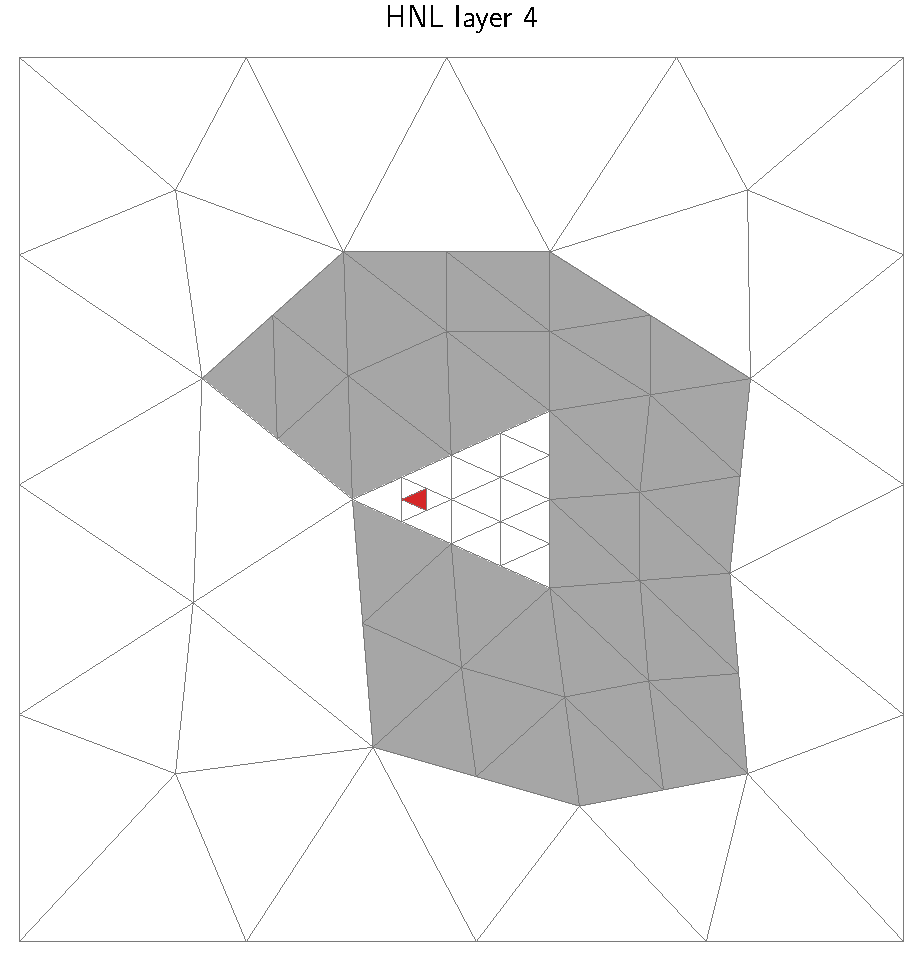
\includegraphics[width=0.31\textwidth]{Fig1d.pdf}\hfill
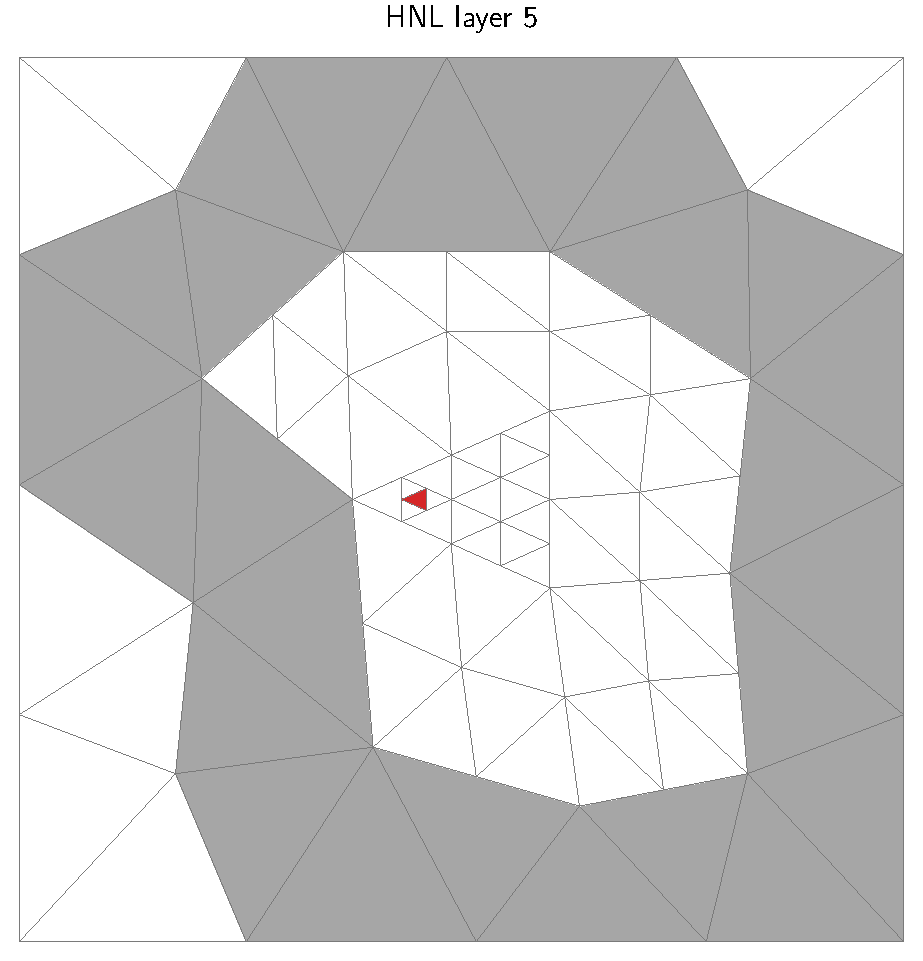
\includegraphics[width=0.31\textwidth]{Fig1e.pdf}\hfill
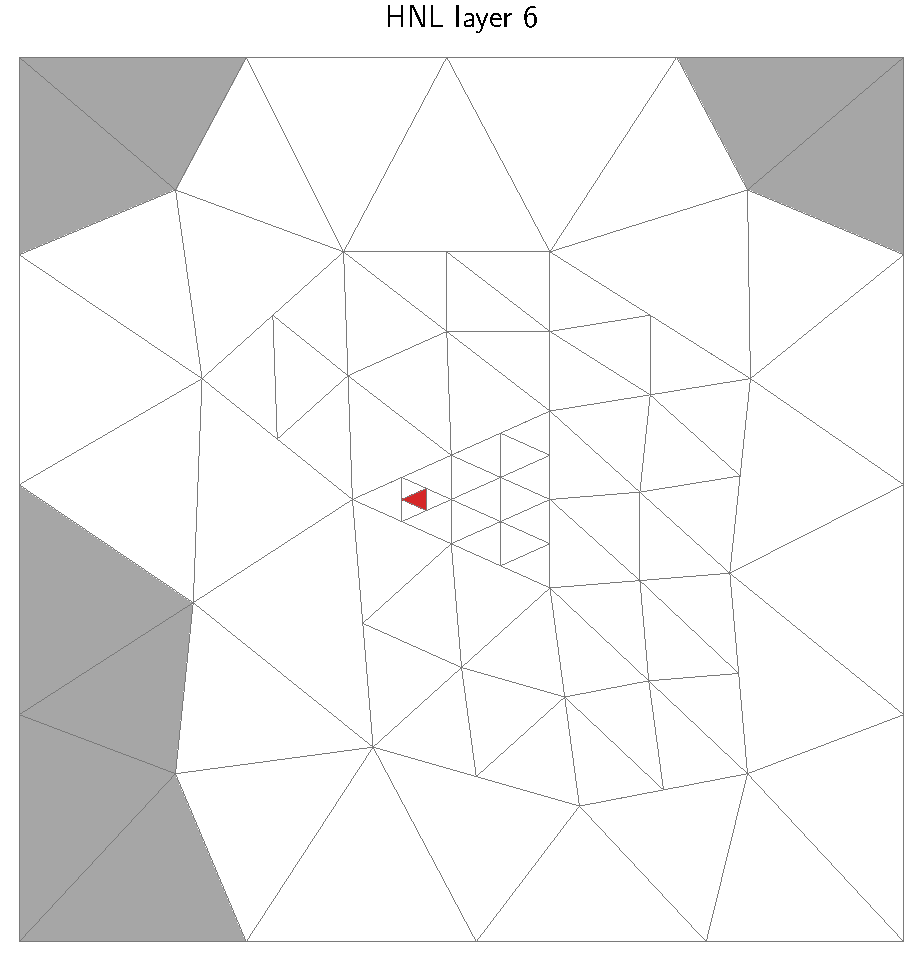
\includegraphics[width=0.31\textwidth]{Fig1f.pdf}
\caption{HNL construction in two dimensions. Panels progress from left to right, then top to bottom. Gray marks the current layer; red marks the target element.}
\label{fig:hnl_layerwise_2d}
\end{figure}

Algorithm~\ref{alg:hnl_expansion} generates candidate regions and materializes their source cover. Write \(\ell(E)\) for the level of element \(E\). Here, \(L_j\) is the current search layer and \(Q\) is the candidate-region set. For an element set \(A\), \(V(A)\) denotes its vertices and \(\operatorname{par}(A)\) its distinct parents; \(\operatorname{sib}(K)\) contains \(K\) and its siblings. The target and all roots are included in \(Q\). At each level, HNL first forms the full vertex-star union and completes the sibling families, then removes the current search-layer elements. Duplicate candidates accumulated across levels are removed separately before materialization. A region with no strict candidate descendant is retained whole; otherwise, it is split recursively into all children. This last step, not the search layers alone, guarantees a complete source cover.

\begin{algorithm}[!htbp]
\SetAlgoLined
\caption{HNL Candidate Search and Source-Cover Construction}

\label{alg:hnl_expansion}
\Input{target leaf $K_t$; root elements $\mathcal R$; level-indexed vertex incidence}
\Output{candidate regions $\mathcal Q$; disjoint source cover $\mathcal C_{K_t}$}
$\mathcal Q\leftarrow\{K_t\}$; $\mathcal L_{\ell(K_t)}\leftarrow\{K_t\}$\;
\For{$j=\ell(K_t),\,\ell(K_t)-1,\ldots,1$}{
  $\mathcal V_j^{\mathrm{front}}\leftarrow
  \operatorname{unique}(\mathcal V(\mathcal L_j))$\;
  $\mathcal E_j\leftarrow
  \displaystyle\bigcup_{v\in\mathcal V_j^{\mathrm{front}}}
  \operatorname{star}_j(v)$\;
  $\mathcal S_j\leftarrow
  \left(\displaystyle\bigcup_{E\in\mathcal E_j}\operatorname{sib}(E)\right)
  \setminus\mathcal L_j$ \tcp{remove the current search-layer elements}
  $\mathcal Q\leftarrow\mathcal Q\cup\mathcal S_j$\;
  $\mathcal L_{j-1}\leftarrow\operatorname{par}(\mathcal L_j\cup\mathcal S_j)$\;
}
$\mathcal Q\leftarrow\operatorname{unique}(\mathcal Q\cup\mathcal R)$\;
$\mathcal C_{K_t}\leftarrow\varnothing$\;
\ForEach{$R\in\mathcal R$}{
  $\mathcal C_{K_t}\leftarrow\mathcal C_{K_t}\cup
  \operatorname{Cover}(R,\mathcal Q)$\;
}
\Return{$\mathcal Q,\mathcal C_{K_t}$}\;
\end{algorithm}


Here, $\operatorname{Cover}(E,\mathcal Q)$ returns $\{E\}$ if $E$ is a leaf or has no strict candidate descendant; otherwise, it returns the union of $\operatorname{Cover}(F,\mathcal Q)$ over all children $F$ of $E$. Root regions are processed independently, so disconnected mesh components are included. Lemma~\ref{lem:hnl_cover} proves that this materialization covers the domain without overlap. Sibling expansion controls where the cover is refined; it is not itself the coverage proof.

Let \(C_{K_t}\) denote the resulting source cover and \(\omega(E)\) the region occupied by the active leaf descendants of \(E\). Complete coverage with nonoverlapping interiors requires
\begin{equation}
\bigcup_{E\in\mathcal C_{K_t}}\omega(E)=\Omega_h,
\qquad
\operatorname{int}\omega(E_i)\cap\operatorname{int}\omega(E_k)=\emptyset
\quad(E_i\ne E_k).
\label{eq:hnl_cover_property}
\end{equation}
Here, \(\Omega_h\) denotes the mesh domain and equals \(\Omega\) in the experiments; shared boundaries are permitted. Lemma~\ref{lem:hnl_cover} establishes this property when roots partition the mesh domain and children partition each refined parent. Lemma~\ref{lem:mac_cover} shows that MAC classification preserves the cover. Appendix~\ref{app:hnl_coverage} gives the proofs and reports independent implementation checks; their costs are excluded from the reported timings.

% Float placement is allowed across subsection boundaries.
\subsection{Multipole Acceptance and Potential Evaluation}
\label{sec:mac}
\label{sec:hartree_evaluation}

HNL constructs the source cover, and the MAC assigns each region to direct integration or multipole evaluation. For each target leaf \(K_t\), accepted clusters form the far-field set \(F(K_t)\), while leaves requiring direct integration form the neighbor set \(N(K_t)\). A rejected internal cluster is replaced by its children, which are tested recursively. Because the children partition their parent, this process preserves source coverage.

The MAC is applied to the entire target leaf, allowing its interaction lists to be shared by all target points within it. Let \((c_t,r_t)\) and \((c_C,R_C)\) denote the centers and radii of enclosing spheres for the target leaf and source cluster \(C\), respectively. Then
\begin{equation}
d_{tC}=|\mathbf c_t-\mathbf c_C|-r_t
\label{eq:target_cluster_distance}
\end{equation}
is a lower bound for \(|x-c_C|\) for all \(x\in K_t\). Cluster \(C\) is accepted when
\begin{equation}
d_{tC}>R_C,\qquad R_C/d_{tC}\leq\theta<1,
\label{eq:geometric_mac}
\end{equation}
where \(\theta\in(0,1)\) controls the required separation. Smaller values impose a stricter acceptance criterion. As illustrated in Figure~\ref{fig:mac_geometry}, this condition ensures convergence of the multipole expansion throughout the target leaf; numerical integration errors are controlled separately.

\begin{figure}[!htbp]
\centering
\resizebox{0.67\textwidth}{!}{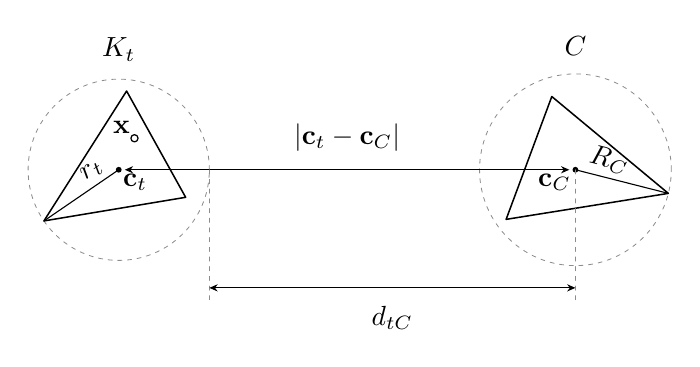
\begin{tikzpicture}[font=\normalsize,line join=round,line cap=round,
  >={Stealth[length=3pt,width=2.6pt]},
  guide/.style={black!45,line width=.3pt,dash pattern=on 1.5pt off 2pt},
  dimension/.style={<->,line width=.38pt}]
  \pgfmathsetmacro{\targetradius}{sqrt(.95*.95+.65*.65)}
  \pgfmathsetmacro{\sourceradius}{sqrt(1.18*1.18+.30*.30)}
  \coordinate (target) at (0,0);
  \coordinate (source) at (5.8,0);
  \coordinate (evaluation) at (.20,.40);
  \coordinate (targetBoundary) at (\targetradius,0);
  \begin{scope}[shift={(target)}]
    \draw[guide] (0,0) circle[radius=\targetradius];
    \draw[line width=.55pt]
      (-.95,-.65)--(.85,-.35)--(.10,1.00)--cycle;
    \draw[line width=.4pt] (0,0)--(-.95,-.65)
      node[pos=.25,sloped,above=1pt,inner sep=1pt] {$r_t$};
  \end{scope}
  \begin{scope}[shift={(source)}]
    \draw[guide] (0,0) circle[radius=\sourceradius];
    \draw[line width=.55pt]
      (-.88,-.63)--(1.18,-.30)--(-.30,.93)--cycle;
    \draw[line width=.4pt] (0,0)--(1.18,-.30)
      node[pos=.32,sloped,above=1pt,inner sep=1pt] {$R_C$};
  \end{scope}
  \node[above=3pt] at (0,\targetradius) {$K_t$};
  \node[above=3pt] at (5.8,\sourceradius) {$C$};
  \draw[dimension,shorten <=2.2pt,shorten >=2.2pt] (target)--(source)
    node[midway,above=3pt] {$|\mathbf c_t-\mathbf c_C|$};
  \fill (target) circle[radius=1.05pt];
  \fill (source) circle[radius=1.05pt];
  \node[below right=2pt,inner sep=0pt] at (target) {$\mathbf c_t$};
  \node[below left=2pt,inner sep=0pt] at (source) {$\mathbf c_C$};
  \begin{scope}[shift={(evaluation)}]
    \draw[fill=white,line width=.45pt] (0,0) circle[radius=1.3pt];
    \node[above left=2pt,inner sep=0pt] at (0,0) {$\mathbf x$};
  \end{scope}
  \draw[guide] (targetBoundary)--(\targetradius,-1.65);
  \draw[guide] (source)--(5.8,-1.65);
  \draw[dimension] (\targetradius,-1.5)--(5.8,-1.5)
    node[midway,below=3pt] {$d_{tC}$};
\end{tikzpicture}
}
\caption{Multipole acceptance geometry. Dashed circles enclose the target leaf and source cluster; $d_{tC}$ bounds the target-to-cluster-center distance from below. Adapted from the layout in \cite[Fig.~1]{Cui}.}
\label{fig:mac_geometry}
\end{figure}

The potential is evaluated by combining direct integration over neighbor leaves with multipole contributions from far-field clusters. Each neighbor leaf is represented by one, two, or four integration tetrahedra. On tetrahedra that do not contain the target, we use a positive-weight Gaussian rule exact for polynomials of total degree up to $p$; thus, $p$ specifies quadrature accuracy rather than the finite element degree. Singular integrals on tetrahedra containing the target are evaluated using the Duffy transformation \cite{Duffy1982}. When analytical subtraction is enabled, the contribution associated with the constant density term is integrated exactly, and Duffy quadrature is applied to the remainder. The treatment used is specified for each experiment.

For each far-field cluster, a Cartesian multipole expansion truncated at total degree $P$ approximates the contribution of its descendant leaves \cite{BeatsonGreengard1997,Cui}. The cluster moments are computed from source quadrature points and density-weighted quadrature weights, then reused by all targets that accept the cluster. Appendix~\ref{app:hartree_evaluation} provides the formulas for regular integration, singular integration, and multipole evaluation.

\subsection{Parallel Implementation and Cost Model}
\label{sec:overall_algorithm}

Algorithm~\ref{alg:hnl_treecode} separates geometry-dependent preprocessing from density-dependent preparation and potential evaluation. For a fixed mesh, geometric data and vertex-to-element adjacency are recorded once, and HNL construction followed by MAC classification produces the interaction lists for each target leaf. List construction and potential evaluation are both parallelized over target leaves. The implementation uses contiguous indexing, per-level vertex stamps, and
thread-local buffers, and stores interaction lists separately for each target
leaf without sharing source covers or merging sibling groups after HNL
construction.

\begin{algorithm}[!htbp]
\caption{Parallel HNL Treecode}
\label{alg:hnl_treecode}
\Input{Adaptive mesh; prescribed source density; target points; quadrature accuracy \(p\); multipole order \(P\); MAC threshold \(\theta\); moment construction and singular integration strategies.}
\Output{Approximate Hartree potential \(V_H^h\) at the target points.}
\tcp{Geometry preprocessing}
Record element geometry, levels, parent and child links, and vertex incidence by level\;
\ForEach{target leaf $K_t$ \textbf{in parallel}}{
  Generate HNL candidates and materialize the complete source cover using Algorithm~\ref{alg:hnl_expansion}.\;
  Apply the MAC recursively to classify source regions into accepted clusters and leaves requiring direct integration.\;
  Store the neighbor list $\mathcal N(K_t)$ and far field list $\mathcal F(K_t)$\;
}
\tcp{Density-dependent preparation}
Cache source quadrature points, weights, and weighted density values\;
\eIf{direct accumulation of cluster moments is selected}{
  Accumulate descendant-leaf quadrature contributions about each cluster center, in parallel over clusters.
}{
  Compute leaf moments in parallel, then translate and accumulate child moments at their parents, proceeding from fine to coarse levels with parallelism within each level.
}
\tcp{Potential evaluation}
\ForEach{target leaf $K_t$ \textbf{in parallel}}{
  \ForEach{target point $\mathbf x\in K_t$}{
    Evaluate neighbor integrals using Gaussian quadrature for regular tetrahedra and Duffy quadrature for singular tetrahedra, with analytical subtraction where enabled.\;
    Add the degree-\(P\) multipole contributions from \(F(K_t)\).\;
    Store the sum as $V_H^h(\mathbf x)$\;
  }
}
\Return{$V_H^h$}\;
\end{algorithm}

We analyze the arithmetic cost using one target per active leaf and assuming constant-cost density evaluation at each source point. Regular integration uses \(q_p=O(p^3)\) quadrature points per tetrahedron, while Duffy quadrature uses \(q=\max(4,\lfloor(p+4)/2\rfloor)\) points in each transformed coordinate. With at most four Duffy subregions per tetrahedron and four integration tetrahedra per leaf, the cost per neighbor interaction is \(O(f(p))\), where
\begin{equation}
f(p)=q_p+4q^3=\mathcal O(p^3).
\label{eq:quadrature_work_factor}
\end{equation}
A Cartesian multipole expansion of total degree \(P\) contains
\begin{equation}
g(P)=N_P=\binom{P+3}{3}
=\mathcal O(P^3).
\label{eq:expansion_work_factor}
\end{equation}
coefficients. With bounded work per coefficient, the evaluation cost per accepted cluster is \(O(g(P))\).

Let \(N_{\mathrm{near}}\) and \(N_{\mathrm{far}}\) denote the total numbers of
neighbor and far-field interactions. Once the moments are available, potential
evaluation costs
\begin{equation}
\mathcal O\!\left(
N_{\mathrm{near}}f(p)+N_{\mathrm{far}}g(P)
\right).
\label{eq:evaluation_complexity}
\end{equation}
How the interaction counts grow with the mesh is examined empirically in
Section~\ref{sec:numerical_experiments}. For a fixed mesh and MAC threshold,
and with moments precomputed, the dependence on the evaluation parameters is
\(O(p^3+P^3)\). Moment preparation has additional coupled dependence on \(p\)
and \(P\), as detailed in Appendix~\ref{app:hartree_evaluation}. Mesh
generation is excluded from this analysis.

\subsection{Quadrature and Multipole Truncation Errors}
\label{sec:error_analysis}

The evaluation error consists of quadrature and multipole truncation
contributions. For a mesh \(\mathcal T_N\) with \(N\) active leaves, write
\(h=\max_{K\in\mathcal T_N}\operatorname{diam}(K)\) and measure the error at
leaf barycenters in the discrete volume-weighted norm
\(\|e\|_{L_h^2}=(\sum_t|K_t||e_t|^2)^{1/2}\), where \(|K_t|\) is the leaf
volume. For each target \(t\), let \(F_{t,f}\) be the Duffy-transformed
singular integrand, with Jacobian, on the unit cube for singular piece \(f\);
let \(T_\alpha\) be the Cartesian kernel coefficient of
Eq.~\eqref{eq:kernel_coefficient}; and let \(\mathcal C_{Q,p}\) be the
remainder constant of the positive-weight rule \(Q_p\), exact through total
degree \(p\) \cite{Stroud1971,DavisRabinowitz1984}. With
\(q=\max(4,\lfloor(p+4)/2\rfloor)\), \(c_q=(q!)^4/((2q+1)[(2q)!]^3)\), and
\(\mathcal R_{p,\alpha,C,\tau}=\mathcal C_{Q,p}\max_{|\beta|=p+1}
\|D^\beta G_{\alpha,C,\tau}\|_{L^\infty(\widehat K)}\) for the mapped moment
integrand \(G_{\alpha,C,\tau}(\widehat{\mathbf y})=|\det D\Phi_\tau|\,
\rho_h(\Phi_\tau(\widehat{\mathbf y}))
(\Phi_\tau(\widehat{\mathbf y})-\mathbf c_C)^\alpha\), define
\begin{align}
S_p
&=|\Omega|^{1/2}c_q\max_t
\sum_f\sum_{\xi\in\{u,v,w\}}
\left\|\partial_\xi^{2q}F_{t,f}\right\|_{L^\infty([0,1]^3)},
\label{eq:main_singular_bound}\\
B_{p,P}
&=|\Omega|^{1/2}\max_t
\sum_{C\in\mathcal F(K_t)}\sum_{|\alpha|\le P}
|T_\alpha(x_t,c_C)|
\sum_{\tau\subset\Omega_C}\mathcal R_{p,\alpha,C,\tau}.
\label{eq:main_moment_bound}
\end{align}
For piecewise-polynomial densities the derivatives in \(\mathcal R\) are taken
elementwise, so \(S_p\) and \(B_{p,P}\) are computable from the density, the
mesh, and the quadrature rule.

\begin{theorem}[Quadrature and multipole truncation errors]
\label{thm:treecode_error}
Let \(\rho_h\in L^1(\Omega)\) with \(\Omega_h=\Omega\); let the mesh hierarchy
have roots that partition \(\Omega\) and children that partition each refined
parent; let the source cover be constructed by
Algorithm~\ref{alg:hnl_expansion} with every accepted cluster satisfying the
MAC~\eqref{eq:geometric_mac}; and let the quadrature rules have positive
weights and be exact through total degree \(p\). If, moreover, the integration
tetrahedra are nondegenerate, the bounding spheres enclose their source and
target regions, the regular integrands are \(C^p\) on each integration
tetrahedron, the mapped moment integrands are piecewise \(C^{p+1}\), and the
Duffy-transformed singular integrands have continuous derivatives through order
\(2q\) in each coordinate, then, in exact arithmetic:
\begin{equation}
\|V_H[\rho_h]-V_H^h\|_{L_h^2}
\le
S_p+B_{p,P}+C_1h^p+C_2\theta^{P+1},
\label{eq:treecode_error_bound}
\end{equation}
where \(S_p\) and \(B_{p,P}\) are defined in Eqs.~\eqref{eq:main_singular_bound} and~\eqref{eq:main_moment_bound}, respectively, and
\begin{equation}
C_1=\frac{8\pi}{3p!}|\Omega|^{1/2}r_*^3M_p,
\qquad
C_2=\frac{|\Omega|^{1/2}\|\rho_h\|_{L^1(\Omega)}}{g_*}.
\label{eq:error_constants}
\end{equation}
Here, \(|\Omega|\) denotes the domain volume, \(r_*\) the maximum near-region radius, \(M_p\) a uniform bound on the absolute values of the \(p\)th directional derivatives of the regular integrands, and \(g_*\) the minimum separation gap among accepted clusters.
\end{theorem}

The coverage and MAC hypotheses of the theorem hold by construction
(Lemmas~\ref{lem:hnl_cover} and~\ref{lem:mac_cover}), and the quadrature
hypotheses hold for the positive-weight Gaussian and Duffy rules used below;
the smoothness hypotheses are assumptions on the density and the mesh. The four
terms of~\eqref{eq:treecode_error_bound} correspond to the four error sources:
\(S_p\) to singular integration, \(B_{p,P}\) to moment quadrature, \(C_1h^p\)
to regular near-field quadrature, and \(C_2\theta^{P+1}\) to multipole
truncation. Appendix~\ref{app:error_bound} derives \(C_1\) from the regular
quadrature remainder and near-region volume, and \(C_2\) from the Coulomb
expansion remainder and MAC separation. These constants depend on the mesh and
interaction lists; the estimate excludes density discretization and domain
truncation errors. The bound distinguishes contributions controlled by
different parameters, indicating why improving a single parameter may
eventually yield limited error reduction. Section~\ref{sec:numerical_experiments}
examines this behavior and the benefits of refining spatial and evaluation
parameters together.

\section{Numerical Experiments}
\label{sec:numerical_experiments}

The numerical experiments assess the accuracy--cost benefits of local refinement, the behavior of single-center and multicenter Gaussian sources, and parallel scalability. At fixed $(p,P,\theta)=(6,4,0.5)$, the finest adaptive mesh has 9.5 times smaller sampled error than the comparable uniform mesh and reduces total runtime by 12.0\%. On the fixed strong-scaling problem, potential evaluation achieves a 57.93-fold speedup with 64 CPU threads. All tests use prescribed sources independently of a complete SCF calculation.

Unless otherwise stated, the computational domain is $\Omega=[-5,5]^3$, and the manufactured potential and source are
\begin{equation}
\label{eq:manufactured_solution}
V_{\mathrm{ex}}(\mathbf x)=\exp(-4\pi x^2-8\pi y^2-12\pi z^2),
\qquad
\rho(\mathbf x)=-\frac{1}{4\pi}\Delta V_{\mathrm{ex}}(\mathbf x),
\end{equation}
where $\mathbf x=(x,y,z)$. The source changes sign and serves as a numerical verification problem rather than a physical electron density. The analytical reference includes the full-space source, whereas the numerical integral is restricted to $\Omega$. Appendix~\ref{app:sampling_truncation} examines the omitted source tails. All tests follow Algorithm~\ref{alg:hnl_treecode} with stored HNL--MAC interaction lists; refinement indicators and evaluation parameters are specified below.

Experiments were performed on two AMD EPYC 7713 processors with 128 physical cores in total and 881 GiB of memory. The code was compiled with GCC 11.4 using \texttt{-O3} and parallelized with OpenMP. Unless otherwise stated, runs use 128 threads with thread binding to cores and dynamic team adjustment disabled, one target per leaf barycenter, and timings that are medians of three runs. We report wall-clock times for list construction, potential evaluation, and the complete calculation as $T_{\mathrm{list}}$, $T_{\mathrm{eval}}$, and $T_{\mathrm{total}}$, respectively. Experiment-specific timing scopes are stated below; independent validation costs are excluded.

Accuracy is measured using the discrete weighted norm
\[
\|v\|_Q=\left(\sum_{j=1}^{M}w_j|v(x_j)|^2\right)^{1/2}.
\]
Here, $Q=\{(x_j,w_j)\}_{j=1}^{M}$, with $w_j>0$ and $\sum_jw_j=|\Omega|$. The absolute and relative errors are
\begin{equation}
\label{eq:sampled_error_measures}
E_Q^{\mathrm{abs}}=\|V_{\mathrm{tree}}-V_{\mathrm{ex}}\|_Q,
\qquad
E_Q^{\mathrm{rel}}=\frac{E_Q^{\mathrm{abs}}}{\|V_{\mathrm{ex}}\|_Q},
\end{equation}
where $V_{\mathrm{tree}}=V_H^h$. Leaf-barycenter sampling uses $Q=\{(x_K,|K|)\}$, with relative error $E_{\mathrm{bar}}$. Mesh-independent validation sets provide complementary estimates, denoted by $E_m^{\mathrm{abs}}$ and $E_m$ at sampling resolution $m$. Their interpretation as continuous $L^2$ errors depends on resolving the spatial error distribution. Appendix~\ref{app:error_checks} describes the sampling and reference checks. Because the sampling measure differs between experiments, each experiment states its own error measure and the error symbols are local to that experiment.

The experiments distinguish the accuracy--cost benefits of local refinement from the effects of the evaluation parameters. Section~\ref{sec:single_center_tests} compares adaptive and uniform meshes on a cube and then tests spherical and tetrahedral domains. Section~\ref{sec:multicenter_tests} presents the three-center test, and Section~\ref{sec:h2o_cluster_experiment} considers the ten-water model. Section~\ref{sec:thread_scaling} examines parallel performance, and Section~\ref{sec:accuracy_parameters} then investigates how quadrature, multipole approximation, and mesh resolution contribute to the observed errors and costs.

% Float placement is allowed across subsection boundaries.
\subsection{Single-Center Tests}
\label{sec:single_center_tests}

\subsubsection{Adaptive versus Uniform Meshes}
\label{sec:adaptive_uniform}

We first assess whether local refinement improves accuracy and cost relative to uniform refinement. Both mesh types evaluate the source in Eq.~\eqref{eq:manufactured_solution} on $\Omega=[-20,20]^3$ using the same HNL--MAC implementation, analytical singularity subtraction, pooled per-leaf storage, 128 CPU threads, and fixed parameters $(p,P,\theta)=(6,4,0.5)$. Uniform meshes contain $N=24\cdot8^\ell$ active leaves after $\ell$ global refinements. Adaptive meshes use the indicator $\int_K|x|^{-1}\,dx$, evaluated with algebraic accuracy six.

Figure~\ref{fig:adaptive_uniform} compares three pairs with similar leaf counts. Adaptive and uniform runs are interleaved within each timing batch. The errors are evaluated at the same $343{,}000$ weighted, mesh-independent targets for every mesh; increasing the target quadrature order from eight to ten changes the reported errors by at most 1.1\%. The separate validation time is excluded from $T_{\mathrm{total}}$.

The coarsest meshes give essentially the same error. On the medium and fine pairs, the adaptive errors are 16.2 and 9.5 times smaller, respectively. The adaptive meshes use 1.8\%, 2.7\%, and 2.0\% fewer leaves and reduce total time by 1.2\%, 8.5\%, and 12.0\%. Thus, at fixed evaluation parameters and comparable $N$, local refinement improves the accuracy--cost trade-off for this localized source.

\begin{figure}[!htbp]
\centering
\resizebox{\textwidth}{!}{%
\begin{tikzpicture}
\begin{groupplot}[
  group style={group size=2 by 1, horizontal sep=0.4cm},
  journalaxis,
  width=0.48\textwidth,
  height=0.45\textwidth,
  xmode=log,ymode=log
]
\nextgroupplot[
  xlabel={$N$},ylabel={$E_Q^{\mathrm{abs}}$},
  legend style={at={(0.98,0.98)},anchor=north east,draw=none,font=\tiny,legend columns=1}
]
\addplot+ coordinates {(12064,5.6474447) (95616,.11628460) (771088,.012194963)};
\addlegendentry{Adaptive}
\addplot+ coordinates {(12288,5.6474547) (98304,1.8891448) (786432,.11625231)};
\addlegendentry{Uniform}
\nextgroupplot[
  xlabel={$N$},ylabel={total time (s)},
  ytick pos=right,
  yticklabel pos=right,
  yticklabel style={xshift=-2pt},
  legend style={at={(0.02,0.98)},anchor=north west,draw=none,font=\tiny,legend columns=1}
]
\addplot+ coordinates {(12064,.792916) (95616,4.836655) (771088,41.382609)};\addlegendentry{Adaptive}
\addplot+ coordinates {(12288,.802672) (98304,5.283108) (786432,47.043884)};\addlegendentry{Uniform}

\end{groupplot}
\end{tikzpicture}%
}
\caption{Absolute error at common targets (left) and total time (right) for
three adaptive and uniform mesh pairs at fixed $(p,P,\theta)=(6,4,0.5)$.
Both axes are logarithmic.}
\label{fig:adaptive_uniform}
\end{figure}

\FloatBarrier

\subsubsection{General-Domain Tests}
\label{sec:general_domain_test}

We next test the method on two non-cubical domains used in general-domain treecode studies \cite{Cui}: the faceted sphere
\[
\Omega_{\mathrm S}=\{\mathbf x\in\mathbb R^3:|\mathbf x|<5\}
\]
and the tetrahedron \(\Omega_{\mathrm T}\) with vertices
\[
(0,0,30),\qquad (20,0,-10),\qquad
(-10,10,-10),\qquad (-10,-10,-10).
\]
On either domain \(\Omega\), we evaluate
\begin{equation}
V_{\Omega}(\mathbf x)=\int_{\Omega}
\frac{\rho(\mathbf y)}{|\mathbf x-\mathbf y|}\,d\mathbf y,
\qquad
\rho(\mathbf y)=\exp\!\left(-4|\mathbf y-\mathbf c|^2\right),
\qquad
\mathbf c=(-2,-2,0).
\label{eq:sphere_gaussian_problem}
\end{equation}
The density is truncated to the computational domain, and the numerical reference is obtained by direct integration on the finest source mesh of the corresponding sequence. Figure~\ref{fig:sphere_tetrahedron_meshes} shows the two starter meshes. Refinement of the sphere subdivides its planar boundary faces without projecting new vertices onto the exact sphere, so that sequence represents a fixed polyhedral approximation of \(\Omega_{\mathrm S}\).

\begin{figure}[!htbp]
\centering
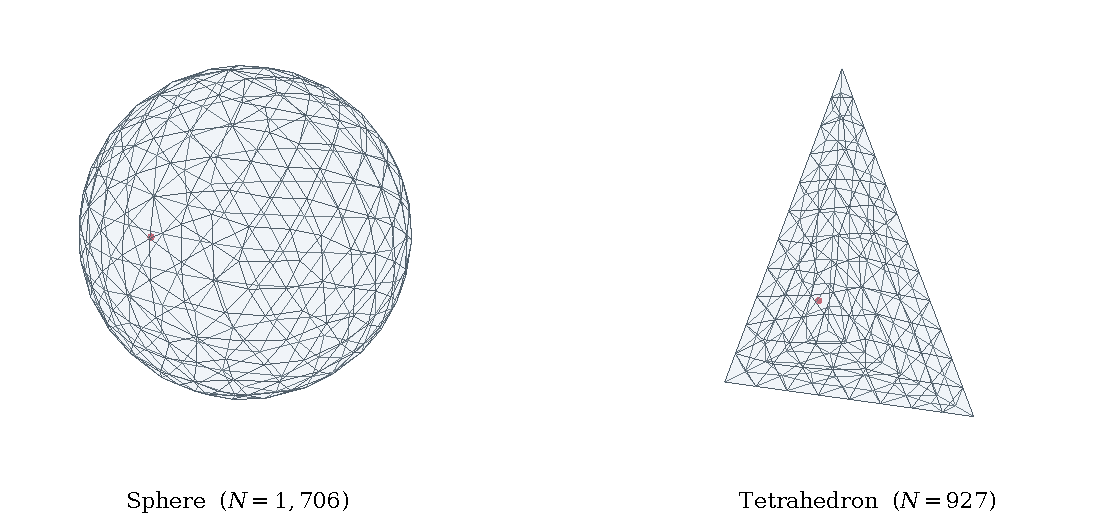
\includegraphics[width=\textwidth]{general_domain/runs/irregular_scaling_p2P4_20261109/sphere_tetrahedron_meshes_3d.pdf}
\caption{Starter tetrahedral meshes for the general-domain tests: the faceted sphere with \(N=1\,706\) (left) and the four-faced tetrahedral domain with \(N=927\) (right). The red point marks the Gaussian center \(\mathbf c=(-2,-2,0)\).}
\label{fig:sphere_tetrahedron_meshes}
\end{figure}

Each sequence contains the starter mesh and three uniform refinements. The sphere uses
\(N=1\,706\), \(13\,648\), \(109\,184\), and \(873\,472\), while the tetrahedron uses
\(N=927\), \(7\,416\), \(59\,328\), and \(474\,624\). All runs use
\((p,P,\theta)=(2,4,0.5)\) and 16 OpenMP threads. We evaluate the potential at the same 128 volume-distributed targets and 32 targets in \(|\mathbf x-\mathbf c|<0.9\) throughout each sequence. For either fixed target set \(G\), the sampled relative error is
\begin{equation}
E_G=\left(
\frac{\sum_{j\in G}|V_j^{\mathrm{tree}}-V_j^{\mathrm{ref}}|^2}
     {\sum_{j\in G}|V_j^{\mathrm{ref}}|^2}
\right)^{1/2}.
\label{eq:sphere_sample_error}
\end{equation}

Figure~\ref{fig:general_domain_scaling} shows decreasing volume and core errors for both geometries. On the finest spherical mesh, \(E_{\mathrm{vol}}=1.29\times10^{-6}\) and \(E_{\mathrm{core}}=2.03\times10^{-6}\); on the finest tetrahedral mesh, the corresponding values are \(6.52\times10^{-7}\) and \(3.50\times10^{-6}\). The complete solver times increase from \(0.088\) to \(121.203\) seconds for the sphere and from \(0.181\) to \(62.619\) seconds for the tetrahedron. Reference evaluation is excluded.

\begin{figure}[!htbp]
\centering
\resizebox{\textwidth}{!}{%
\begin{tikzpicture}
\begin{groupplot}[
  group style={group size=2 by 1, horizontal sep=0.4cm},
  journalaxis,
  width=0.48\textwidth,
  height=0.45\textwidth,
  xmode=log,
  ymode=log
]
\nextgroupplot[
  xlabel={$N$},
  ylabel={sampled relative error},
  legend style={at={(0.02,0.02)},anchor=south west,draw=none,font=\tiny,legend columns=1}
]
\addplot[blue,mark=*] coordinates {
  (1706,1.258e-3) (13648,2.449e-4) (109184,1.822e-5) (873472,1.290e-6)
};\addlegendentry{Sphere: \(E_{\mathrm{vol}}\)}
\addplot[blue,dashed,mark=square*] coordinates {
  (1706,6.129e-3) (13648,1.369e-3) (109184,2.336e-4) (873472,2.034e-6)
};\addlegendentry{Sphere: \(E_{\mathrm{core}}\)}
\addplot[orange,mark=triangle*] coordinates {
  (927,4.246e-2) (7416,5.064e-4) (59328,8.036e-5) (474624,6.517e-7)
};\addlegendentry{Tetrahedron: \(E_{\mathrm{vol}}\)}
\addplot[orange,dashed,mark=diamond*] coordinates {
  (927,5.198e-2) (7416,5.864e-3) (59328,1.005e-3) (474624,3.505e-6)
};\addlegendentry{Tetrahedron: \(E_{\mathrm{core}}\)}
\nextgroupplot[
  xlabel={$N$},
  ylabel={total time (s)},
  ytick pos=right,
  yticklabel pos=right,
  yticklabel style={xshift=-2pt},
  legend style={at={(0.02,0.98)},anchor=north west,draw=none,font=\tiny}
]
\addplot[blue,mark=*] coordinates {
  (1706,.088) (13648,.979) (109184,11.737) (873472,121.203)
};\addlegendentry{Sphere}
\addplot[orange,mark=triangle*] coordinates {
  (927,.181) (7416,.433) (59328,5.691) (474624,62.619)
};\addlegendentry{Tetrahedron}
\end{groupplot}
\end{tikzpicture}%
}
\caption{General-domain refinement results at \((p,P,\theta)=(2,4,0.5)\) using 16 OpenMP threads. Left: sampled relative errors on the volume-distributed and source-core target sets. Right: complete solver time. Both axes in each panel are logarithmic.}
\label{fig:general_domain_scaling}
\end{figure}

\FloatBarrier

We next examine whether the method retains its accuracy for sources with multiple localized centers.

% Float placement is allowed across subsection boundaries.
\subsection{Multicenter Test}
\label{sec:multicenter_tests}

To extend the single-center comparison to multiple localized regions, we consider a three-center manufactured problem based on H$_2$O geometry. Three Gaussian potentials are placed at the atomic positions in $\Omega=[-5,5]^3$, with coordinates in bohr given by
\[
\mathbf R_{\mathrm O}=(0,0,0),\qquad
\mathbf R_{\mathrm H_1}=(1.43043,0,1.10716),\qquad
\mathbf R_{\mathrm H_2}=(-1.43043,0,1.10716).
\]
For each center $R_A=(X_A,Y_A,Z_A)$, $A\in\{\mathrm O,\mathrm H_1,\mathrm H_2\}$, define the Gaussian potential and its manufactured source as
\[
u_A(\mathbf x)=
\exp\!\left[-4\pi(x-X_A)^2-8\pi(y-Y_A)^2
-12\pi(z-Z_A)^2\right],
\qquad
f_A=-\frac{1}{4\pi}\Delta u_A.
\]
By linearity, the total source and analytical reference potential are
\[
f(\mathbf x)=\sum_A f_A(\mathbf x),
\qquad
u_{\mathrm{ex}}(\mathbf x)=\sum_Au_A(\mathbf x).
\]
The numerical integral is restricted to the computational cube, as in the single-center test.

A single tetrahedral mesh resolves all three centers using element integrals of
\[
I_{\mathrm{all}}(\mathbf x)
=\max_{A\in\{\mathrm O,\mathrm H_1,\mathrm H_2\}}
\frac{1}{|\mathbf x-\mathbf R_A|}.
\]
The combined source is evaluated with the same list construction and potential evaluation routines as before, without target sharing. Analytical singularity subtraction is applied within 0.25 bohr of an atomic center; elsewhere, Duffy quadrature treats the full singular integrand. Figure~\ref{fig:h2o_single_all_atom_mesh} illustrates the local refinement pattern.

Figure~\ref{fig:h2o_single_mesh_n_scaling} jointly increases $N$, $p$, and $P$ at fixed $\theta=0.5$, using $(p,P)=(4,2),(6,4),(8,6),(10,8)$ in increasing-$N$ order. Runs use four OpenMP threads. Total time includes mesh and moment preparation, list construction, and potential evaluation, but excludes final error accumulation. The mesh panels in Figure~\ref{fig:h2o_single_all_atom_mesh} are illustrative snapshots, not the full four-mesh sequence used for this convergence curve.

\begin{figure}[!htbp]
\centering
\makebox[\textwidth][c]{%
  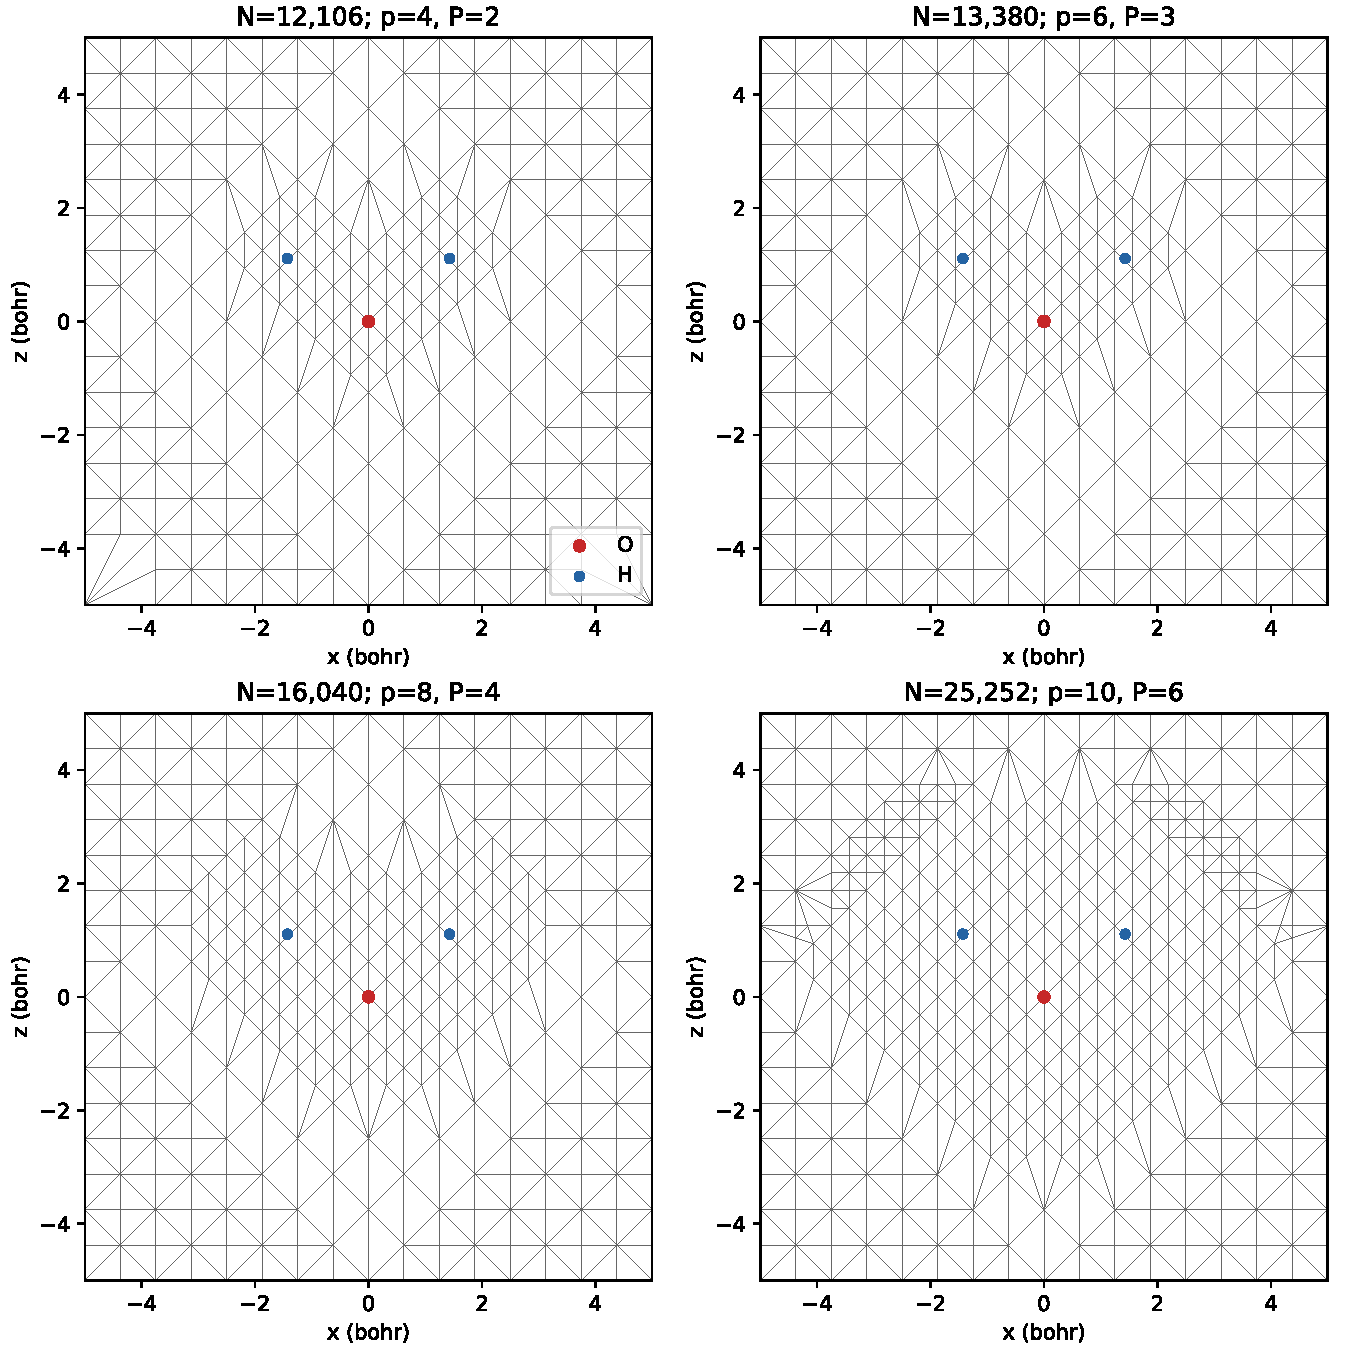
\includegraphics[width=1.08\textwidth]{arxiv_figures/single_h2o_meshes.pdf}}
\caption{Illustrative adaptive meshes for the three-center manufactured problem, shown in cuts at $y\approx0$. Red and blue markers denote projected O and H positions. Panel labels give $N$, $p$, and $P$; $N$ counts active leaf macroelements. These snapshots illustrate the refinement pattern and are not the full sequence in Figure~\ref{fig:h2o_single_mesh_n_scaling}.}
\label{fig:h2o_single_all_atom_mesh}
\end{figure}

Joint refinement reduces the relative volume-weighted barycenter error from $5.6565\times10^{-2}$ to $2.9178\times10^{-5}$, as shown in Figure~\ref{fig:h2o_single_mesh_n_scaling}. The accompanying runtime increase reflects both mesh refinement and higher evaluation orders. We next consider a nonnegative source distributed over 30 atomic centers. The separate three-center sampling study in Appendix~\ref{app:sampling_truncation} assesses target-sampling sensitivity and does not validate this mesh sequence directly.

\begin{figure}[!htbp]
\centering
\resizebox{\textwidth}{!}{%
\begin{tikzpicture}
\begin{groupplot}[
  group style={group size=2 by 1, horizontal sep=0.4cm},
  journalaxis,
  width=0.48\textwidth,
  height=0.45\textwidth,
  xmode=log,
  grid=major,
  tick label style={font=\small},
  label style={font=\small},
  title style={font=\small}
]
\nextgroupplot[
  title={Barycenter relative error},xlabel={$N$},
  ymode=log,
  ylabel={$E_{L^2}^{\mathrm{bar}}$}
]
\addplot+[thick] coordinates {
  (12106,5.6565e-2)
  (49122,6.2771e-4)
  (106116,8.5134e-5)
  (180687,2.9178e-5)
};
\nextgroupplot[
  title={Total solver time},xlabel={$N$},
  ymode=log,
  ytick pos=right,
  yticklabel pos=right,
  yticklabel style={xshift=-2pt},
  ylabel={$T_{\mathrm{total}}$ (s)}
]
\addplot+[thick] coordinates {
  (12106,1.336)
  (49122,15.423)
  (106116,67.107)
  (180687,251.931)
};
\end{groupplot}
\end{tikzpicture}%
}
\caption{Single-H$_2$O joint refinement. Left: relative volume-weighted
error at leaf barycenters. Right: total time, including list
construction, preparation, and potential evaluation.}
\label{fig:h2o_single_mesh_n_scaling}
\end{figure}

% Float placement is allowed across subsection boundaries.
\subsection{Ten-Water Gaussian Source Model}
\label{sec:h2o_cluster_experiment}

The ten-water test uses a nonnegative Gaussian source at the 30 atomic positions of a water cluster. The geometry is taken from the TIP4P $(\mathrm{H_2O})_{10}$ configuration in the Cambridge Cluster Database \cite{CambridgeTIP4P10,WalesHodges1998}, translated to center its atomic bounding box at the origin, and converted to bohr. The prescribed density is
\begin{equation}
\label{eq:h2o_cluster_density}
\rho(\mathbf x)=\sum_{a=1}^{30}q_a
\left(\dfrac{\alpha_a}{\pi}\right)^{3/2}
\exp\!\left[-\alpha_a|\mathbf x-\mathbf R_a|^2\right],
\end{equation}
where $\mathbf R_a$ denotes the position of atom $a$, with $(q_a,\alpha_a)=(8,2)$ for oxygen and $(1,1)$ for hydrogen in atomic units. The density integrates to 100 over all space and is independent of an SCF calculation. Its analytical free-space potential is
\begin{equation}
\label{eq:h2o_cluster_reference}
V_{\mathrm{ex}}(\mathbf x)=\sum_{a=1}^{30}q_a
\dfrac{\operatorname{erf}(\sqrt{\alpha_a}|\mathbf x-\mathbf R_a|)}
{|\mathbf x-\mathbf R_a|}.
\end{equation}
At $\mathbf x=\mathbf R_a$, the corresponding potential term has the finite limit $2q_a\sqrt{\alpha_a/\pi}$.

The computational domain extends the atomic bounding box by 4 bohr in each direction, giving
\[
\Omega\simeq[-9.3962,9.3962]\times[-10.1619,10.1619]
\times[-10.4273,10.4273].
\]
As in the preceding tests, the reference retains the full-space source tails; the omitted source integral is approximately $4.75\times10^{-8}$. Local refinement uses element integrals of the regularized multicenter monitor
\begin{equation}
\label{eq:h2o_cluster_monitor}
m(\mathbf x)=\dfrac{1}{30}\sum_{a=1}^{30}
\left[|\mathbf x-\mathbf R_a|^2+\delta^2\right]^{-1/2},
\qquad \delta=0.5\ \text{bohr}.
\end{equation}

After one initial global refinement, the mesh is adapted using monitor quadrature of algebraic accuracy six, independently of $p$. The implementation uses per-leaf interaction lists, direct accumulation of cluster moments, and analytical singularity subtraction at every target. Figure~\ref{fig:h2o_cluster_convergence} jointly increases $N$, $p$, and $P$ at fixed $\theta=0.5$; Figure~\ref{fig:h2o_cluster_mesh_sequence} shows the meshes. Runs use four OpenMP threads without target sharing. Reported times include barycenter error accumulation, but exclude geometry loading, domain mesh-file generation, and independent validation.

Errors are evaluated on a fixed stratified target set shared by all meshes. Each target $x_j$ represents a subbox $B_j$ and receives the volume weight $w_j=|B_j|$; the reported relative discrete error is
\[
E=\left(\frac{\sum_j |B_j|\,|V_{\mathrm{tree}}(x_j)-V_{\mathrm{ex}}(x_j)|^2}
 {\sum_j |B_j|\,|V_{\mathrm{ex}}(x_j)|^2}\right)^{1/2}.
\]
A second target set assesses sampling sensitivity. Barycenter errors $E_{\mathrm{bar}}$ are reported separately to show how the estimate depends on target placement.

\begin{figure}[!htbp]
\centering
\makebox[\textwidth][c]{%
  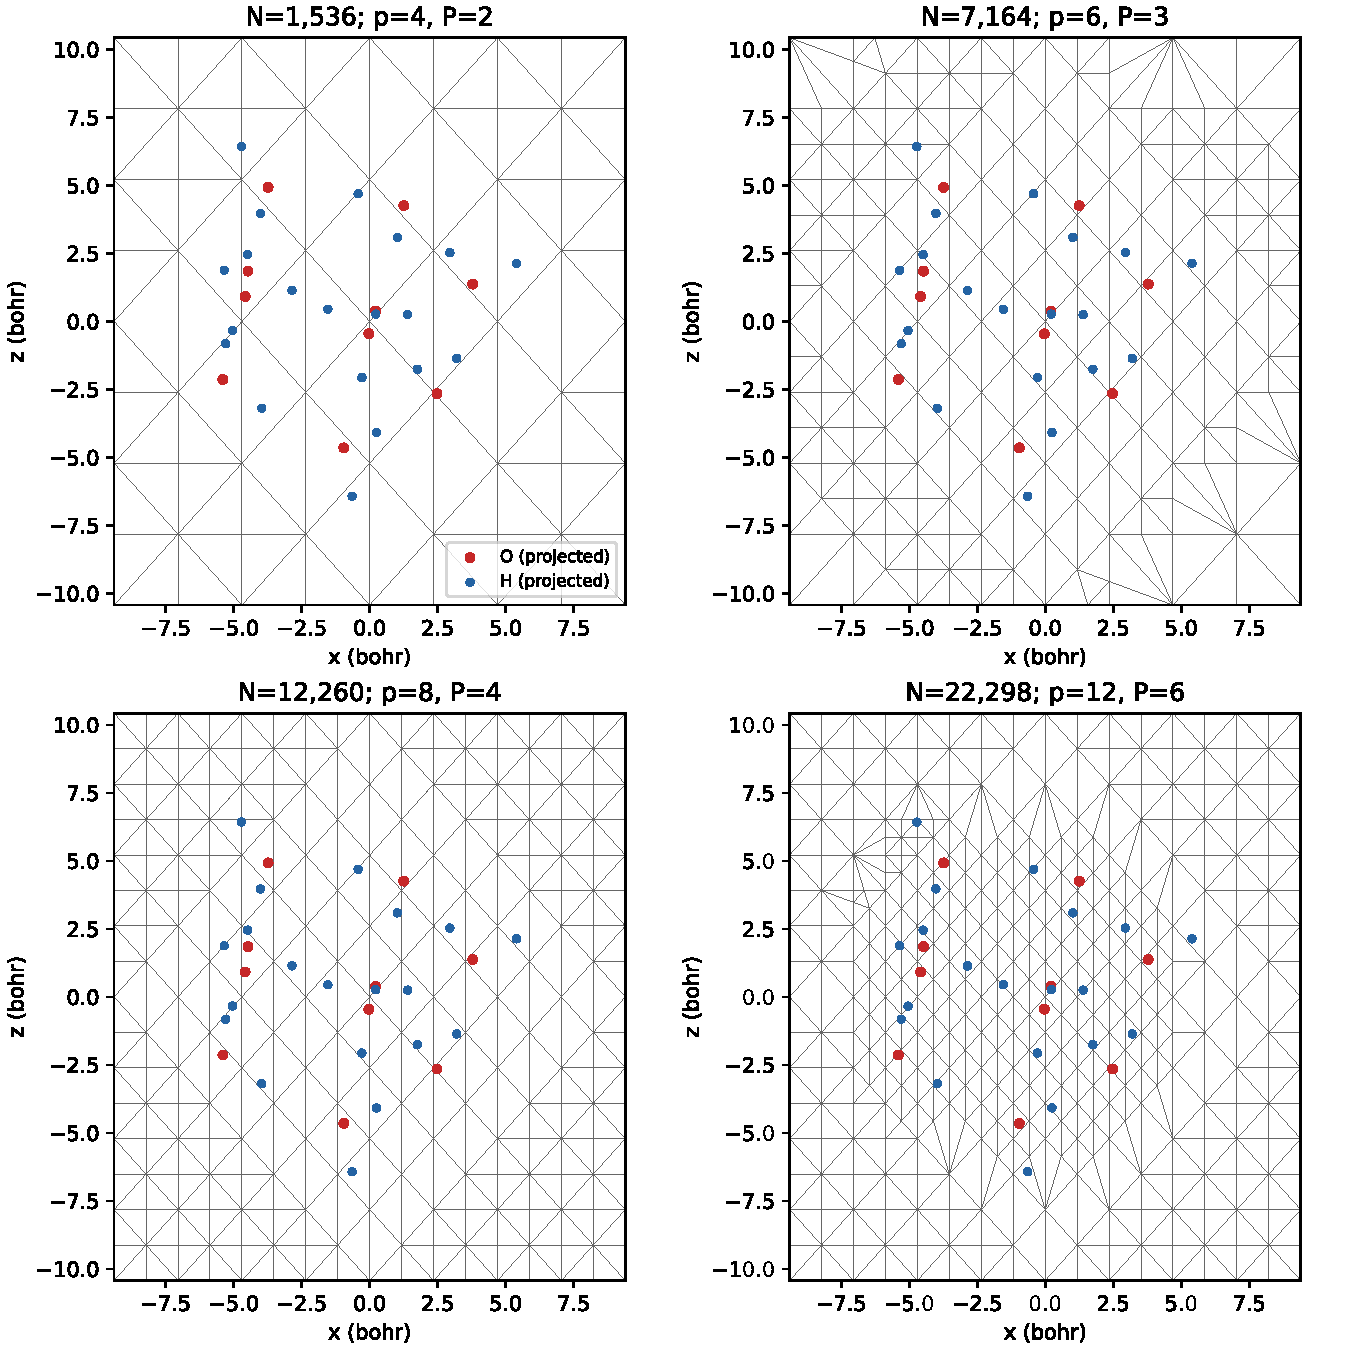
\includegraphics[width=1.08\textwidth]{arxiv_figures/ten_h2o_meshes.pdf}}
\caption{Adaptive meshes for the ten-water Gaussian source model, shown in cuts at $y=10^{-6}$ bohr. Red and blue markers denote projected O and H positions. Composite leaves are decomposed for visualization; $N$ counts active leaf macroelements.}
\label{fig:h2o_cluster_mesh_sequence}
\end{figure}

\begin{figure}[!htbp]
\centering
\resizebox{\textwidth}{!}{%
\begin{tikzpicture}
\begin{groupplot}[
  group style={group size=2 by 1, horizontal sep=0.4cm},
  journalaxis,
  width=0.48\textwidth,
  height=0.45\textwidth,
  xmode=log, ymode=log
]
\nextgroupplot[xlabel={$N$},ylabel={$E$}]
\addplot+ coordinates {
  (1536,1.048e-2)
  (7164,3.530e-4)
  (12260,2.252e-4)
  (22298,2.375e-5)
};
\nextgroupplot[
  xlabel={$N$}, ylabel={seconds},
  ytick pos=right,
  yticklabel pos=right,
  yticklabel style={xshift=-2pt},
  legend style={at={(0.02,0.98)},anchor=north west,draw=none,font=\tiny,legend columns=1}
]
\addplot+ coordinates {
  (1536,0.008) (7164,0.077)
  (12260,0.122) (22298,0.342)
};
\addlegendentry{List}

\addplot+ coordinates {
  (1536,0.124) (7164,1.515)
  (12260,4.182) (22298,22.876)
};
\addlegendentry{Evaluation}

\addplot+ coordinates {
  (1536,0.183) (7164,1.886)
  (12260,5.060) (22298,27.486)
};
\addlegendentry{Total}
\end{groupplot}
\end{tikzpicture}%
}

\caption{Joint refinement for the H$_2$O cluster.
Left: relative sampled error $E$ on the common target set.
In increasing $N$ order,
$(p,P)=(4,2),(6,3),(8,4),(12,6)$.
Right: median interaction list, potential evaluation,
and total solver times. Both $p$ and $P$ increase
with $N$, so this timing curve is not a complexity
study at fixed orders.}
\label{fig:h2o_cluster_convergence}
\end{figure}

For this 30-center source, joint refinement reduces $E$ from $1.048\times10^{-2}$ to $2.375\times10^{-5}$, an approximately 441-fold reduction (Figure~\ref{fig:h2o_cluster_convergence}). The second validation set changes the estimate by at most 6.4\% across the four meshes and by 3.1\% on the finest mesh. Together with the three-center test, these results demonstrate improved sampled accuracy under joint refinement for both manufactured and nonnegative multicenter sources. We next examine the parallel performance of potential evaluation.

% Float placement is allowed across subsection boundaries.
\subsection{Strong Scaling}
\label{sec:thread_scaling}

The target evaluations are independent, so we measure strong scaling on a fixed problem: the $N=100\,432$ mesh, leaf-barycenter targets, and $(p,P,\theta)=(6,4,0.5)$. Per-target interaction lists remain fixed as the thread count changes. We test $N_{\mathrm{th}}\in\{1,2,4,8,16,32,64\}$. Each setting is run three times in separate processes with varied run order. The absolute volume-weighted barycenter error is $2.1886\times10^{-4}$ for all settings. Runs use \texttt{OMP\_PLACES=cores} and \texttt{OMP\_PROC\_BIND=close}; the 2- and 4-thread timings are from a later batch of the same executable, checked against the 8-thread result.

Figure~\ref{fig:thread_scaling} shows median evaluation times and the speedup $S_{\mathrm{eval}}(t)=T_{\mathrm{eval}}(1)/T_{\mathrm{eval}}(t)$. Speedup is close to ideal through 32 threads and reaches 57.93 at 64 threads, corresponding to 90.5\% parallel efficiency. The figure measures potential evaluation only, not list construction or the complete solver.


\begin{figure}[!htbp]
\centering
\resizebox{\textwidth}{!}{%
\begin{tikzpicture}
\begin{groupplot}[
  group style={group size=2 by 1, horizontal sep=0.4cm},
  journalaxis,
  width=0.48\textwidth,
  height=0.45\textwidth,
  xmin=0, xmax=66,
  xtick={1,16,32,64}
]
\nextgroupplot[
  xlabel={$N_{\mathrm{th}}$},
  ylabel={$T_{\mathrm{eval}}$ (s)},
  ymode=log
]
\addplot+ coordinates {
  (1,162.096)
  (2,80.654)
  (4,40.278)
  (8,20.155)
  (16,10.119)
  (32,5.085)
  (64,2.798)
};
\nextgroupplot[
  xlabel={$N_{\mathrm{th}}$},
  ylabel={speedup},
  ymode=normal,
  ytick pos=right,
  yticklabel pos=right,
  yticklabel style={xshift=-2pt},
  xmin=0, xmax=66,
  ymin=0, ymax=66,
  xtick={1,16,32,64},
  legend style={
    at={(0.02,0.98)},
    anchor=north west,
    legend columns=1,
    font=\tiny,
    draw=none
  }
]
\addplot+ coordinates {
  (1,1.000)
  (2,2.010)
  (4,4.024)
  (8,8.042)
  (16,16.019)
  (32,31.877)
  (64,57.933)
};
\addlegendentry{Measured}

\addplot[dashed,black,mark=none] coordinates {
  (1,1) (64,64)
};
\addlegendentry{Ideal}
\end{groupplot}
\end{tikzpicture}%
}

\caption{CPU evaluation time and speedup using the original
per-target-list storage with 1--64 threads on a fixed source
mesh and target set. Left: median evaluation time
$T_{\mathrm{eval}}$ over three runs.
Right: speedup
$S_{\mathrm{eval}}(t)=T_{\mathrm{eval}}(1)/T_{\mathrm{eval}}(t)$;
the dashed line indicates ideal speedup.
Both horizontal axes are linear; the time axis is logarithmic
and the speedup axis is linear.}
\label{fig:thread_scaling}
\end{figure}

\FloatBarrier

% Float placement is allowed across subsection boundaries.
\subsection{Parameter Sensitivity and Error Analysis}
\label{sec:accuracy_parameters}

The preceding experiments establish the practical accuracy--cost benefits and parallel performance of the method. We now examine the parameter choices underlying these results. Fixed-mesh sweeps isolate the effects of quadrature accuracy, multipole order, and the MAC threshold; mesh refinement and reference-based error decomposition then identify the limits of improving any one component alone.

% Float placement is allowed across subsection boundaries.
\subsubsection{Evaluation Parameters}
\label{sec:parameter_saturation}

To separate evaluation effects from mesh changes, we use a fixed adaptive mesh with $N=100\,432$ active leaves. It is generated from 24 coarse elements using the single-center indicator of Section~\ref{sec:adaptive_uniform}, evaluated independently of $p$. Varying $p$, $P$, or $\theta$ therefore leaves the source mesh unchanged.

The parameter sweeps in Figure~\ref{fig:parameter_error_plateaus} share the baseline $(p,P,\theta)=(6,4,0.5)$, with analytical singularity subtraction at every target. Here, $E_h$ denotes the absolute volume-weighted barycenter error. The mesh-refinement study below uses the same execution settings.

We first vary $p$ at fixed $P=4$ and $\theta=0.5$. This changes regular, singular, and moment quadrature without altering the interaction lists.

Quadrature refinement initially reduces the error substantially, but its benefit diminishes at higher $p$ (Figure~\ref{fig:parameter_error_plateaus}). Increasing $p$ from 8 to 12 reduces $E_h$ by only 5.3\%, while increasing $T_{\mathrm{eval}}$ by a factor of 2.62. List construction time remains approximately constant because the interaction lists are unchanged.

% Float placement is allowed across subsection boundaries.
We next vary $P$ at fixed $p=6$ and $\theta=0.5$. The coefficient count $N_P=\binom{P+3}{3}$ grows with the expansion order, increasing moment construction and far-field evaluation costs while leaving the interaction lists unchanged.

A similar saturation occurs when increasing the multipole order (Figure~\ref{fig:parameter_error_plateaus}). Raising $P$ from 6 to 8 reduces $E_h$ by only 0.74\%, while increasing $T_{\mathrm{eval}}$ by a factor of 1.84. Higher orders therefore offer limited improvement in the sampled total error at these settings.

% Float placement is allowed across subsection boundaries.
Finally, we vary $\theta$ at fixed $p=6$ and $P=4$. A smaller threshold imposes stricter separation, causing further subdivision of rejected clusters and generally increasing the number of interactions.

Tightening the MAC produces the same pattern of diminishing returns (Figure~\ref{fig:parameter_error_plateaus}). Reducing $\theta$ from 0.3 to 0.2 decreases $E_h$ by only 0.26\%, while increasing $T_{\mathrm{eval}}$ by a factor of 2.81. The additional far-field accuracy therefore yields little improvement in the sampled total error.

\begin{figure}[!htbp]
\centering
\resizebox{\textwidth}{!}{%
\begin{tikzpicture}
\begin{groupplot}[
  journalaxis,
  group style={
    group size=2 by 3,
    horizontal sep=0.8cm,
    vertical sep=0.9cm
  },
  width=0.48\textwidth,
  height=0.32\textwidth,
  tick label style={font=\scriptsize},
  label style={font=\scriptsize}
]

% Row 1: quadrature accuracy p
\nextgroupplot[
  xlabel={$p$},
  ylabel={$E_h$},
  ymode=log
]
\addplot+ coordinates {
  (2,.023569)
  (4,.0012447)
  (6,.00021886)
  (8,.00016025)
  (12,.00015177)
};

\nextgroupplot[
  xlabel={$p$},
  ylabel={seconds},
  ytick pos=right,
  yticklabel pos=right,
  yticklabel style={xshift=-2pt},
  ymin=0,ymax=12,
  legend style={at={(0.02,0.98)},anchor=north west,draw=none,font=\tiny,legend columns=1}
]
\addplot+ coordinates {
  (2,.992) (4,.990) (6,1.084)
  (8,1.013) (12,1.060)
};
\addlegendentry{List}
\addplot+ coordinates {
  (2,1.077) (4,1.213) (6,1.471)
  (8,1.939) (12,5.075)
};
\addlegendentry{Evaluation}
\addplot+ coordinates {
  (2,3.532) (4,3.854) (6,4.292)
  (8,5.376) (12,9.628)
};
\addlegendentry{Total}

% Row 2: multipole order P
\nextgroupplot[
  xlabel={$P$},
  ylabel={$E_h$},
  ymode=log
]
\addplot+ coordinates {
  (2,.0020987)
  (4,.00021886)
  (6,.00015787)
  (8,.00015671)
};

\nextgroupplot[
  xlabel={$P$},
  ylabel={seconds},
  ytick pos=right,
  yticklabel pos=right,
  yticklabel style={xshift=-2pt},
  ymin=0,ymax=10
]
\addplot+ coordinates {
  (2,1.020) (4,1.084) (6,.931) (8,.911)
};
\addplot+ coordinates {
  (2,.855) (4,1.471) (6,2.853) (8,5.249)
};
\addplot+ coordinates {
  (2,3.821) (4,4.292) (6,5.830) (8,8.248)
};

% Row 3: MAC threshold theta
\nextgroupplot[
  xlabel={$\theta$},
  ylabel={$E_h$},
  ymode=log
]
\addplot+ coordinates {
  (.2,.00015668)
  (.3,.00015709)
  (.5,.00021886)
  (.7,.00057681)
};

\nextgroupplot[
  xlabel={$\theta$},
  ylabel={seconds},
  ytick pos=right,
  yticklabel pos=right,
  yticklabel style={xshift=-2pt},
  ymin=0,ymax=20
]
\addplot+ coordinates {
  (.2,1.710) (.3,1.533) (.5,1.084) (.7,.770)
};

\addplot+ coordinates {
  (.2,12.633) (.3,4.494) (.5,1.471) (.7,.811)
};

\addplot+ coordinates {
  (.2,16.334) (.3,8.012) (.5,4.292) (.7,3.420)
};

\end{groupplot}
\end{tikzpicture}
}%

\caption{HNL parameter sweeps on the same $N=100\,432$
mesh. Rows from top to bottom vary quadrature accuracy
$p$, multipole order $P$, and MAC threshold $\theta$,
respectively. Left: absolute volume-weighted
leaf-barycenter error on logarithmic vertical axes.
Right: median list construction, potential evaluation,
and total times; the legend in the top-right panel applies
to all three timing panels. All horizontal axes are linear.
Fixed parameters are stated in the text preceding each sweep.}
\label{fig:parameter_error_plateaus}
\end{figure}

Figure~\ref{fig:parameter_error_plateaus} summarizes a common outcome: improving one evaluation parameter eventually adds substantial cost with little reduction in total error. The sweeps are consistent with competing contributions in Eq.~\eqref{eq:treecode_error_bound}, but do not identify them individually. Before separating those contributions, we examine the effect of mesh resolution.

% Float placement is allowed across subsection boundaries.

% Float placement is allowed across subsection boundaries.
\subsubsection{Mesh Resolution}
\label{sec:experiment_n}

To isolate the effect of spatial resolution, we refine the cubic single-center mesh at fixed $(p,P,\theta)=(6,4,0.5)$, retaining the same initial mesh, indicator, and indicator quadrature accuracy. Figure~\ref{fig:single_center_five_meshes} shows representative coarse and fine meshes; these snapshots are illustrative and are not the five meshes plotted in Figure~\ref{fig:single_center_hnl_scaling}.

\begin{figure}[!htbp]
\centering
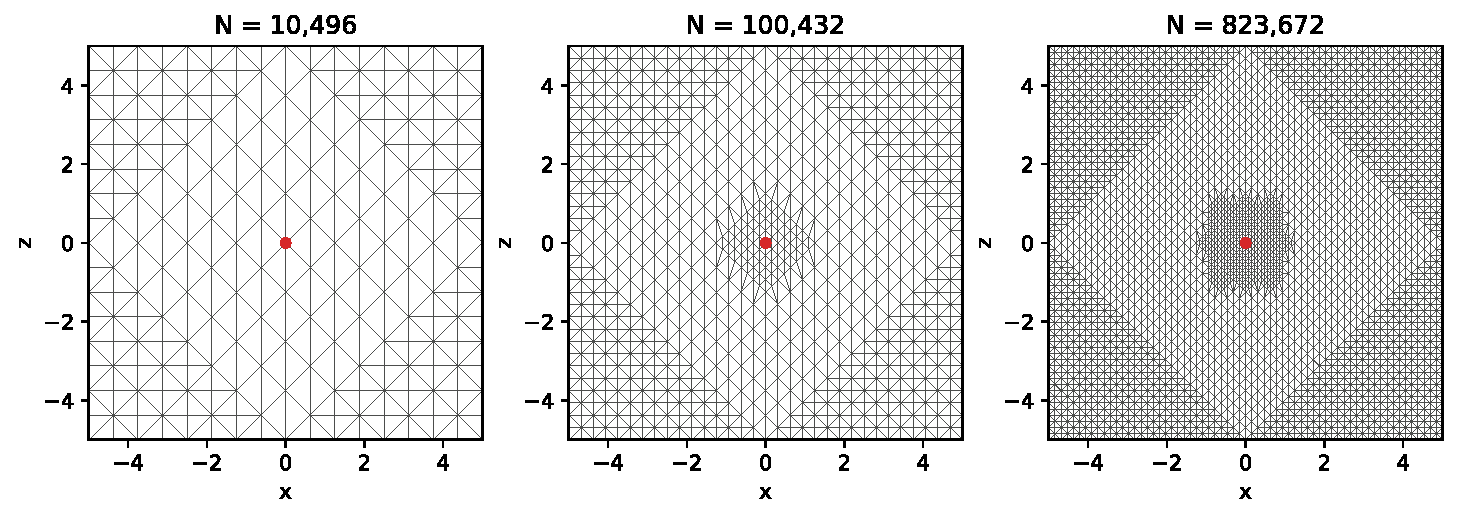
\includegraphics[
  width=0.48\textwidth,
  trim={0pt 0pt 465pt 0pt},
  clip
]{arxiv_figures/single_center_meshes.pdf}\hfill
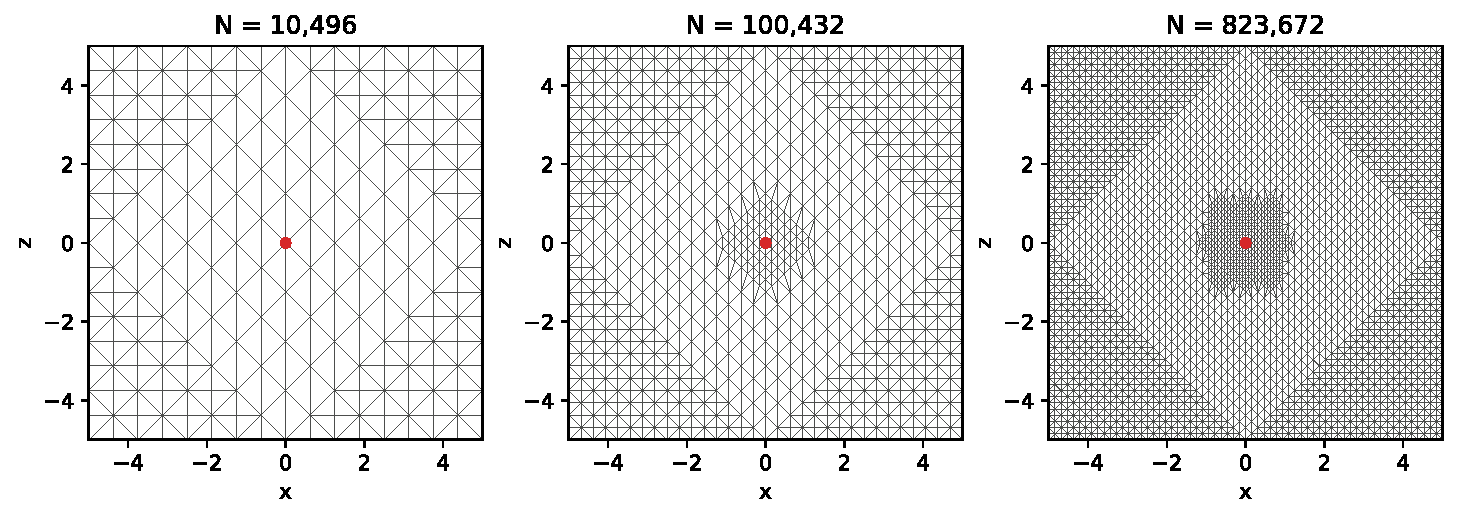
\includegraphics[
  width=0.48\textwidth,
  trim={465pt 0pt 0pt 0pt},
  clip
]{arxiv_figures/single_center_meshes.pdf}
\caption{Coarse and fine single-center adaptive meshes, shown in cuts at $y=10^{-6}$; the panels are labeled by their element counts. The source center is marked in red. These snapshots illustrate the refinement pattern and are not the five data points in Figure~\ref{fig:single_center_hnl_scaling}.}
\label{fig:single_center_five_meshes}
\end{figure}

The error $E_h$ is evaluated at leaf barycenters against the analytical reference in Eq.~\eqref{eq:manufactured_solution}. Because these targets change with the mesh, Appendix~\ref{app:sampling_truncation} provides complementary checks on mesh-independent target sets. Mesh refinement reduces the sampled error rapidly over the first three meshes, after which it remains near $2\times10^{-4}$ (Figure~\ref{fig:single_center_hnl_scaling}). Both list construction and evaluation costs increase with refinement. The normalized $N\log N$ line illustrates the measured runtime growth and is not a fitted complexity law.

\begin{figure}[!htbp]
\centering
\resizebox{\textwidth}{!}{%
\begin{tikzpicture}
\begin{groupplot}[
  journalaxis,
  group style={group size=2 by 1, horizontal sep=0.4cm},
  width=0.48\textwidth,
  height=0.45\textwidth,
  xmode=log,
  grid=major,
  tick label style={font=\sffamily\small},
  label style={font=\sffamily\small}
]
\nextgroupplot[
  xlabel={$N$},
  ymode=log,
  ylabel={$E_{L^2}$}
]
\addplot+[thick] coordinates {
  (10160,5.6610e-2)
  (35920,1.1495e-3)
  (100656,2.1886e-4)
  (192888,1.6778e-4)
  (423034,1.7555e-4)
};
\nextgroupplot[
  xlabel={$N$},
  ymode=log,
  ytick pos=right,
  yticklabel pos=right,
  yticklabel style={xshift=-2pt},
  ylabel={seconds},
  legend style={at={(0.02,0.98)},anchor=north west,draw=none,font=\tiny,legend columns=1}
]
\addplot+[thick] coordinates {
  (10160,0.534)
  (35920,2.151)
  (100656,5.568)
  (192888,13.213)
  (423034,32.925)
};
\addlegendentry{measured}
\addplot[dashed,black,thick] coordinates {
  (10160,0.534)
  (35920,2.146)
  (100656,6.605)
  (192888,13.373)
  (423034,31.221)
};
\addlegendentry{normalized $N\log N$}
\end{groupplot}
\end{tikzpicture}%
}
\caption{Cubic-domain mesh-refinement results at $(p,P,\theta)=(6,4,0.5)$. Left: absolute barycenter error. Right: total runtime and an $N\log N$ reference normalized at the smallest mesh.}
\label{fig:single_center_hnl_scaling}
\end{figure}

Together with the fixed-mesh parameter sweeps, this result shows that improving one component alone can eventually give little reduction in the total error. We next separate the principal error contributions.

% Float placement is allowed across subsection boundaries.
\subsubsection{Error Decomposition}
\label{sec:error_validation}

We use reference calculations to determine which contributions limit further error reduction. Keeping the HNL--MAC interaction partition fixed, we separate singular quadrature, regular near-field quadrature, moment quadrature, and multipole truncation errors. These correspond to the contributions bounded by $S_p$, $C_1h^p$, $B_{p,P}$, and $C_2\theta^{P+1}$ in Theorem~\ref{thm:treecode_error}. Figure~\ref{fig:four_error_terms} reports numerical estimates of the components rather than their theoretical bounds.

The decomposition uses the $N=100\,432$ mesh, $\theta=0.5$, and 64 CPU threads. All curves use the same 77 selected leaf barycenters with leaf-volume weights; the resulting norms diagnose this target set rather than the full domain. Higher-order quadrature supplies reference neighbor integrals and moments, while direct integration supplies the accepted far-field contributions without multipole truncation. Reference refinement changes each checked component norm by less than 0.17\%. Appendix~\ref{app:error_checks} gives the reference rules and signed differences.

\begin{figure}[!htbp]
\centering
\resizebox{\textwidth}{!}{%
\begin{tikzpicture}
\begin{groupplot}[
  group style={group size=2 by 1, horizontal sep=0.4cm},
  journalaxis,
  width=0.48\textwidth,
  height=0.45\textwidth,
  ymode=log,
  grid=major,
  tick label style={font=\sffamily\small},
  label style={font=\sffamily\small},
  title style={font=\sffamily\small},
  legend style={at={(0.02,0.02)},anchor=south west,draw=none,font=\tiny,legend columns=1},
  ymax=3e-3
]
\nextgroupplot[
  title={Fixed $P=4$, $\theta=0.5$},
  xlabel={Quadrature accuracy $p$},
  ylabel={Weighted norm $\|e\|_Q$},
  xmin=3.6, xmax=12.4,
  xtick={4,6,8,12},
  ymin=3e-11,
  ymax=3e-3,
  ytick={1e-9,1e-7,1e-5,1e-3}
]
\addplot+ coordinates {(4,2.030e-5) (6,7.497e-6) (8,2.911e-6) (12,2.926e-7)};
\addlegendentry{Singular}
\addplot+ coordinates {(4,1.318e-4) (6,3.769e-5) (8,1.361e-5) (12,2.258e-6)};
\addlegendentry{Regular}
\addplot+ coordinates {(4,4.878e-5) (6,1.775e-6) (8,5.903e-8) (12,5.538e-11)};
\addlegendentry{Moment}
\addplot+ coordinates {(4,2.571e-6) (6,2.571e-6) (8,2.571e-6) (12,2.571e-6)};
\addlegendentry{Truncation}
\addplot+ coordinates {(4,1.248e-4) (6,3.278e-5) (8,1.207e-5) (12,3.286e-6)};
\addlegendentry{Total signed}

\nextgroupplot[
  title={Fixed $p=6$, $\theta=0.5$},
  xlabel={Multipole order $P$},
  ytick pos=right,
  yticklabel pos=right,
  yticklabel style={xshift=-2pt},
  xmin=1.8, xmax=8.2,
  xtick={2,4,6,8},
  ymin=2e-8, ymax=7e-5,
  ytick={1e-7,1e-6,1e-5}
]
\addplot+ coordinates {(2,7.499e-6) (4,7.499e-6) (6,7.499e-6) (8,7.499e-6)};
\addplot+ coordinates {(2,3.770e-5) (4,3.770e-5) (6,3.770e-5) (8,3.770e-5)};
\addplot+ coordinates {(2,1.774e-6) (4,1.774e-6) (6,1.775e-6) (8,1.775e-6)};
\addplot+ coordinates {(2,3.673e-5) (4,2.571e-6) (6,4.416e-7) (8,4.570e-8)};
\addplot+ coordinates {(2,4.920e-5) (4,3.279e-5) (6,3.272e-5) (8,3.272e-5)};
\end{groupplot}
\end{tikzpicture}%
}
\caption{Error decomposition at $N=100\,432$. Left: $p$ varies with $P=4$ and $\theta=0.5$ fixed. Right: $P$ varies with $p=6$ and $\theta=0.5$ fixed. Legend entries denote singular and regular near-field quadrature, moment quadrature, multipole truncation, and total signed error against direct summation. Norms use 77 fixed volume-weighted leaf barycenters; the total is the norm of the signed sum, not the sum of component norms.}
\label{fig:four_error_terms}
\end{figure}

At fixed $P=4$, increasing $p$ from 4 to 12 reduces all three quadrature components, while the multipole truncation contribution remains approximately $2.57\times10^{-6}$. By $p=12$, regular quadrature and truncation errors are comparable on the selected targets. This explains why quadrature refinement alone provides progressively less improvement.

At fixed $p=6$, increasing $P$ from 2 to 8 reduces the truncation contribution from $3.67\times10^{-5}$ to $4.57\times10^{-8}$, while leaving the quadrature contributions essentially unchanged. The total error remains near $3.27\times10^{-5}$ for $P\geq4$, indicating a quadrature-dominated regime on these targets. Thus, higher multipole order alone cannot remove the observed plateau.

The observed plateaus depend on both the parameter choices and the error sampling. In the independent common-target study in Appendix~\ref{app:sampling_truncation}, Table~\ref{tab:target_refinement}, errors decrease across all three source meshes; the final target refinement changes the estimates by less than 2.2\%. This sequence differs from Figure~\ref{fig:single_center_hnl_scaling} in both meshes and sampling. The direct-summation checks in Figure~\ref{fig:error_components} provide additional diagnostics at fixed quadrature. These validation studies support the interpretation of the measured errors without implying a universal convergence rate.

\subsubsection{Multicenter Parameter Check}
\label{sec:multicenter_parameter_check}

The same parameter dependence appears in the ten-water model. At $(p,P,\theta)=(6,4,0.5)$, the relative barycenter errors are $1.983\times10^{-5}$ and $2.042\times10^{-5}$ for $N=22\,298$ and $98\,304$, respectively. On the latter mesh, increasing only $p$ to 10 reduces the error to $8.215\times10^{-6}$, whereas increasing only $P$ to 8 gives $1.901\times10^{-5}$. Using $(p,P,\theta)=(10,8,0.3)$ reduces it further to $2.626\times10^{-6}$, with an evaluation time of 269.591 s. These barycenter estimates use a different sampling measure from Figure~\ref{fig:h2o_cluster_convergence}, but reinforce the same practical conclusion: mesh resolution and evaluation parameters must be coordinated to obtain additional accuracy efficiently.

% Float placement is allowed across subsection boundaries.
\section{Conclusions}
\label{sec:conclusions}

We have developed a treecode algorithm for Hartree potential evaluation on locally refined tetrahedral meshes. By reusing the mesh refinement hierarchy, HNL organizes candidate regions from fine to coarse levels, and recursive materialization gives a complete source cover with nonoverlapping interiors. The MAC then determines whether each region is evaluated by direct integration or multipole approximation. The error analysis distinguishes singular, regular, and moment quadrature errors from multipole truncation error, clarifying the roles of mesh resolution and evaluation parameters.

Numerical experiments demonstrate the accuracy and efficiency of the method for the prescribed single-center and multicenter sources on cubical domains. Additional tests on a faceted sphere and a tetrahedral domain illustrate its use on non-cubical geometries. The parameter studies show that improving one evaluation parameter can yield diminishing error reduction once other contributions dominate, motivating coordinated refinement of spatial resolution, quadrature accuracy, and multipole order. At fixed evaluation parameters and comparable leaf counts, the localized-source test shows that adaptive meshes achieve a more favorable accuracy--cost trade-off than uniform meshes using the same evaluator. Reference calculations identify the competing error contributions and demonstrate the importance of mesh-independent validation targets. Potential evaluation achieves a 57.93-fold speedup on 64 CPU threads, corresponding to 90.5\% parallel efficiency on the tested problem.

Future work will focus on error-guided parameter selection and on reducing
interaction-list construction and storage costs. Two extensions are directly
connected to the motivation given above. Coupling the evaluator to a Kohn--Sham
solver will allow its effect on SCF convergence and total energies to be
measured, together with comparisons against Poisson solvers under matched
accuracy and computational conditions. Real-time time-dependent Kohn--Sham
propagation is a second target: the potential is then required at every time
step while the mesh is usually held fixed, so reusing the geometric data and
interaction lists across density updates directly reduces the cost per step.
When the mesh is updated, whether between SCF iterations or during propagation,
the same separation of geometry and density suggests updating the affected lists
incrementally instead of rebuilding them globally, and determining the mesh
update frequency at which this remains profitable is part of that investigation.
Neither extension has been carried out here; the present experiments assess the
evaluator on prescribed densities, independently of a self-consistent or
time-dependent calculation.

\appendix
\section{Evaluation Details, Error Analysis, and Proofs}
\label{app:theory}
\label{app:evaluation_validation}

\subsection{Quadrature and Multipole Evaluation}
\label{app:hartree_evaluation}

Density values are evaluated directly at source quadrature points; the prescribed analytical sources are not replaced by polynomial interpolants. Let $K_t$ contain the target $\mathbf x$, and let $\mathcal T_{\mathrm{near}}(K_t)$ contain the tetrahedral pieces of its neighbor leaves. We distinguish singular and regular pieces by
\begin{equation}
\mathcal S(\mathbf x)=
\{\tau\in\mathcal T_{\mathrm{near}}(K_t):\mathbf x\in\overline\tau\},
\qquad
\mathcal R(\mathbf x)=
\mathcal T_{\mathrm{near}}(K_t)\setminus\mathcal S(\mathbf x).
\label{eq:singular_set}
\end{equation}
A mesh leaf may contribute to both sets; the closure includes targets on piece boundaries. Hats below denote quadrature approximations.

For $\tau\in\mathcal S(\mathbf x)$, analytical subtraction separates the integrable Coulomb singularity:
\begin{equation}
\begin{aligned}
\int_\tau\frac{\rho_h(\mathbf r')}{|\mathbf x-\mathbf r'|}\,d\mathbf r'
&=\rho_h(\mathbf x)J_\tau(\mathbf x)+I_\tau^{\mathrm{reg}}(\mathbf x),\\
J_\tau(\mathbf x)&=\int_\tau\frac{1}{|\mathbf x-\mathbf r'|}\,d\mathbf r',\\
I_\tau^{\mathrm{reg}}(\mathbf x)&=\int_\tau
\frac{\rho_h(\mathbf r')-\rho_h(\mathbf x)}{|\mathbf x-\mathbf r'|}\,d\mathbf r'.
\end{aligned}
\label{eq:singular_split}
\end{equation}
The geometric integral $J_\tau$ is evaluated analytically by a polyhedral potential formula \cite{Werner1994}. The remainder is integrated by Duffy quadrature: the tetrahedron is partitioned into pieces with $\mathbf x$ as a vertex, each mapped to a standard simplex where a tensor-product Gauss rule applies \cite{Duffy1982}. Without subtraction, the same transformation treats the full singular integrand.

For $\tau\in\mathcal R(\mathbf x)$, collapsed-coordinate Gaussian quadrature gives
\begin{equation}
\label{eq:near_gaussian}
\widehat I_{\tau}^{\mathrm{dir}}(\mathbf x)
=
\sum_{q=1}^{q_p}
w_{\tau,q}
\frac{\rho_h(\mathbf r_{\tau,q})}
     {|\mathbf x-\mathbf r_{\tau,q}|},
\end{equation}
where $\mathbf r_{\tau,q}$ and $w_{\tau,q}$ include the mapping Jacobian, and
\[
q_p=
\left\lfloor\frac{p+4}{2}\right\rfloor
\left\lfloor\frac{p+3}{2}\right\rfloor
\left\lfloor\frac{p+2}{2}\right\rfloor
\]
points give exactness for polynomials of total degree at most $p$. The near-field contribution $V_{\mathrm{near}}^h(\mathbf x)$ sums \eqref{eq:near_gaussian} over $\mathcal R(\mathbf x)$, and the singular contribution $V_{\mathrm{sing}}^h(\mathbf x)$ sums $\rho_h(\mathbf x)J_\tau(\mathbf x)+\widehat I_\tau^{\mathrm{reg}}(\mathbf x)$ over $\mathcal S(\mathbf x)$.

For an accepted cluster $C$ with descendant-leaf region $\Omega_C$ and expansion center $\mathbf c_C$, the exact moment and its quadrature approximation are
\begin{equation}
\label{eq:multipole_moment}
M_\alpha(C)
=
\int_{\Omega_C}
\rho_h(\mathbf r')
(\mathbf r'-\mathbf c_C)^\alpha
\,d\mathbf r',
\qquad
|\alpha|\le P,
\end{equation}
\[
\widehat M_\alpha(C)=
\sum_{\substack{\tau\text{ an integration piece}\\\tau\subset\Omega_C}}
\sum_{q=1}^{q_p}w_{\tau,q}\rho_h(\mathbf r_{\tau,q})
(\mathbf r_{\tau,q}-\mathbf c_C)^\alpha.
\]

Moments are formed by direct accumulation of leaf samples or by exact child-to-parent translation of retained moments; the single-center and ten-water tests use the former and the three-center test the latter. Moment preparation costs $\mathcal O(Nq_pg(P)(L+1))$ for hierarchy depth $L$, plus $\mathcal O(NPg(P))$ for translation.

The Cartesian kernel coefficient is
\begin{equation}
\label{eq:kernel_coefficient}
T_\alpha(\mathbf x,\mathbf c_C)
=
\frac{1}{\alpha!}
\left.
D_{\mathbf y}^{\alpha}
\frac{1}{|\mathbf x-\mathbf y|}
\right|_{\mathbf y=\mathbf c_C},
\end{equation}
where differentiation is with respect to the source variable. The computed far-field contribution is
$V_{\mathrm{far}}^h(\mathbf x)=\sum_{C\in\mathcal F(K_t)}\sum_{|\alpha|\le P}
T_\alpha(\mathbf x,\mathbf c_C)\widehat M_\alpha(C)$.
The total potential is $V_H^h=V_{\mathrm{sing}}^h+V_{\mathrm{near}}^h+V_{\mathrm{far}}^h$; interaction lists follow Sections~\ref{sec:hnl} and~\ref{sec:mac}.

\subsection{Error Decomposition and Validation Checks}
\label{app:error_checks}

The reference studies distinguish fast-summation effects, individual error components, and target-sampling sensitivity. Higher-order integration provides the component references. Direct comparisons and target-refinement checks use 128 threads, and the four-component checks use 64. Validation costs are excluded from solver timings.

On the $N=100\,432$ mesh, let $D_p$ denote direct summation with the same source quadrature and singular rule as the treecode, but without MAC classification or multipole approximation. At identical targets,
\[
V_{\mathrm{tree}}-V_{\mathrm{ex}}
=(V_{\mathrm{tree}}-D_p)+(D_p-V_{\mathrm{ex}}),\qquad
E_Q^{\mathrm{abs}}\leq
\|V_{\mathrm{tree}}-D_p\|_Q+\|D_p-V_{\mathrm{ex}}\|_Q.
\]
The first difference measures the fast-summation effect at fixed quadrature, including numerical moment errors; the second contains quadrature and source-truncation errors. This split does not separately identify $S_p$, $B_{p,P}$, and $C_1h^p$.

Figure~\ref{fig:error_components} shows the three differences on 4096 common weighted targets (seed 7351); because the sampled reference norm differs from the analytical norm by about $20\%$, these are target-set diagnostics rather than resolved continuous norms. At $(p,P,\theta)=(6,4,0.5)$ the treecode--direct and direct--analytical differences are $1.57\times10^{-4}$ and $5.51\times10^{-4}$; raising $P$ to 8 or tightening $\theta$ to 0.2 reduces the former to $3.23\times10^{-6}$ and $1.16\times10^{-6}$, while raising $p$ from 2 to 12 reduces the latter from $2.38\times10^{-2}$ to $1.10\times10^{-4}$. An independent target set with seed 19477 reproduces this behavior.

\begin{figure}[!htbp]
\centering
\resizebox{\textwidth}{!}{%
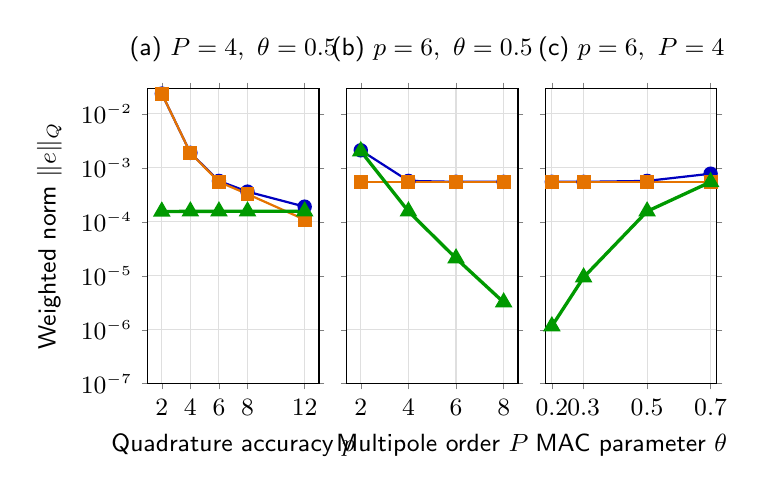
\begin{tikzpicture}

\begin{groupplot}[
  group style={
    group size=3 by 1,
    horizontal sep=0.35cm
  },
  width=0.31\textwidth,
  height=0.44\textwidth,
  ymode=log,
  log basis y=10,
  ymin=1e-7,
  ymax=3e-2,
  ytick={1e-7,1e-6,1e-5,1e-4,1e-3,1e-2},
  grid=major,
  grid style={gray!25},
  axis line style={black},
  tick align=outside,
  major tick length=2pt,
  minor tick length=1pt,
  tick label style={font=\sffamily\small},
  label style={font=\sffamily\small},
  title style={font=\sffamily\small},
  legend style={draw=none,font=\tiny,legend columns=1}
]

% -------------------------------------------------
% Quadrature accuracy p
% -------------------------------------------------
\nextgroupplot[
  title={(a) \(P=4,\ \theta=0.5\)},
  xlabel={Quadrature accuracy \(p\)},
  ylabel={Weighted norm $\|e\|_Q$},
  xtick={2,4,6,8,12},
  legend to name=errorComponentsLegend,
  legend style={draw=none,font=\footnotesize,legend columns=3,column sep=0.45cm}
]

\addplot[
  blue!75!black,
  solid,
  thick,
  mark=*,
  mark size=2.2pt
]
coordinates {
  (2,  2.3789019313406913e-2)
  (4,  1.8979342406881263e-3)
  (6,  5.7385413846022000e-4)
  (8,  3.6278569325222500e-4)
  (12, 1.9136209369358882e-4)
};
\addlegendentry{Treecode--analytical}

\addplot[
  orange!90!black,
  solid,
  thick,
  mark=square*,
  mark size=2.1pt
]
coordinates {
  (2,  2.3777390183921780e-2)
  (4,  1.8980864667093344e-3)
  (6,  5.5128129303267550e-4)
  (8,  3.2726811165467934e-4)
  (12, 1.0996904545299078e-4)
};
\addlegendentry{Direct--analytical}

\addplot[
  green!60!black,
  solid,
  very thick,
  mark=triangle*,
  mark size=2.5pt
]
coordinates {
  (2,  1.5548700518898972e-4)
  (4,  1.5662711899331095e-4)
  (6,  1.5665221088851053e-4)
  (8,  1.5665188011357360e-4)
  (12, 1.5665175193652035e-4)
};
\addlegendentry{Treecode--direct}

% -------------------------------------------------
% Multipole order P
% -------------------------------------------------
\nextgroupplot[
  title={(b) \(p=6,\ \theta=0.5\)},
  xlabel={Multipole order \(P\)},
  yticklabel=\empty,
  xtick={2,4,6,8},
]

\addplot[
  blue!75!black,
  solid,
  thick,
  mark=*,
  mark size=2.2pt
]
coordinates {
  (2, 2.1171925044881222e-3)
  (4, 5.7385413846022000e-4)
  (6, 5.5168948084285110e-4)
  (8, 5.5129734616395900e-4)
};

\addplot[
  orange!90!black,
  solid,
  thick,
  mark=square*,
  mark size=2.1pt
]
coordinates {
  (2, 5.5128129303267550e-4)
  (4, 5.5128129303267550e-4)
  (6, 5.5128129303267550e-4)
  (8, 5.5128129303267550e-4)
};

\addplot[
  green!60!black,
  solid,
  very thick,
  mark=triangle*,
  mark size=2.5pt
]
coordinates {
  (2, 2.0436300680182254e-3)
  (4, 1.5665221088851053e-4)
  (6, 2.1100330297935130e-5)
  (8, 3.2275439079890534e-6)
};

% -------------------------------------------------
% MAC parameter theta
% -------------------------------------------------
\nextgroupplot[
  title={(c) \(p=6,\ P=4\)},
  xlabel={MAC parameter \(\theta\)},
  yticklabel=\empty,
  xtick={0.2,0.3,0.5,0.7},
  xmin=0.18,
  xmax=0.72
]

\addplot[
  blue!75!black,
  solid,
  thick,
  mark=*,
  mark size=2.2pt
]
coordinates {
  (0.2, 5.5128925188854920e-4)
  (0.3, 5.5140997228275850e-4)
  (0.5, 5.7385413846022000e-4)
  (0.7, 7.8040389920778200e-4)
};

\addplot[
  orange!90!black,
  solid,
  thick,
  mark=square*,
  mark size=2.1pt
]
coordinates {
  (0.2, 5.5128129303267550e-4)
  (0.3, 5.5128129303267550e-4)
  (0.5, 5.5128129303267550e-4)
  (0.7, 5.5128129303267550e-4)
};

\addplot[
  green!60!black,
  solid,
  very thick,
  mark=triangle*,
  mark size=2.5pt
]
coordinates {
  (0.2, 1.1646337616854534e-6)
  (0.3, 9.3748216855474570e-6)
  (0.5, 1.5665221088851053e-4)
  (0.7, 5.4908328101350340e-4)
};
\end{groupplot}
\end{tikzpicture}%
}
\par\vspace{-1mm}\centering\pgfplotslegendfromname{errorComponentsLegend}\par


\caption{Direct-summation error diagnostics at $N=100\,432$, evaluated on 4096 common weighted targets. Panels (a)--(c) vary $p$, $P$, and $\theta$, respectively; all use the same logarithmic vertical scale. The shared legend is below the panels. Component norms need not sum to the total because signed errors can cancel.}
\label{fig:error_components}
\end{figure}

% Float placement is allowed across subsection boundaries.
For the four-component decomposition, retain each target's HNL--MAC partition. Let $I_{\mathrm s,p}$ and $I_{\mathrm r,p}$ denote singular and regular neighbor sums, $F_{p,P}$ the expansion using quadrature moments, and $D_{\mathrm f}^{\mathrm{ref}}$ direct integration over accepted far-field regions. Superscript $\mathrm{ref}$ denotes higher-order integration on the same regions. The signed differences are
\begin{equation}
\begin{aligned}
e_{\mathrm s}&=I_{\mathrm s,p}-I_{\mathrm s}^{\mathrm{ref}},&
e_{\mathrm r}&=I_{\mathrm r,p}-I_{\mathrm r}^{\mathrm{ref}},\\
e_{\mathrm b}&=F_{p,P}-F_{\mathrm{ref},P},&
e_{\mathrm t}&=F_{\mathrm{ref},P}-D_{\mathrm f}^{\mathrm{ref}}.
\end{aligned}
\label{eq:four_error_differences}
\end{equation}
Their sum equals $V_{\mathrm{tree}}-V^{\mathrm{ref}}$, where $V^{\mathrm{ref}}=I_{\mathrm s}^{\mathrm{ref}}+I_{\mathrm r}^{\mathrm{ref}}+D_{\mathrm f}^{\mathrm{ref}}$. They estimate the contributions bounded by $S_p$, $C_1h^p$, $B_{p,P}$, and $C_2\theta^{P+1}$, respectively; their norms need not add.

The decomposition uses 77 selected leaf barycenters (nearest to $\{-0.6,-0.2,0.2,0.6\}^3$, the origin, and twelve axial points at distances $1.5$ and $4$) with leaf-volume weights, so the norms characterize only this target set. Reference regular quadrature and moments use algebraic accuracies 28 and 36, and singular quadrature uses 24 and 32 Duffy nodes; across 17 checks on the $N=10\,496$ and $100\,432$ meshes, reference refinement changes each component norm by less than $0.17\%$, and the higher-order direct reference differs from the analytical potential by at most $6.5\times10^{-9}$ on the selected targets. Conservative derivative bounds for the theoretical terms substantially exceed the measured components and are not practical accuracy predictors here; these finite tests do not certify the reference integrals or establish a global $h^p$ rate.

\label{app:sampling_truncation}
Validation targets are generated independently of the source mesh by dividing the domain into subboxes, placing one reproducible seeded point in each subbox, and weighting it by the subbox volume; targets and seeds remain fixed along each refinement curve.

For the single-center sampling check, the approximation is fixed while the validation targets are refined ($m=16,32,64$ inner subintervals per coordinate, two seeds pooled in Table~\ref{tab:target_refinement}): the final refinement changes the estimates by less than $2.2\%$, the finest-resolution seeds differ by less than $1.9\%$, and the finest pooled reference norm differs from the analytical value by about $0.12\%$. Target placement affects the inferred trend: a set of $786\,432$ uniform barycenters reverses the ordering of the last two meshes in Table~\ref{tab:target_refinement}, so target count alone need not resolve errors concentrated near the Gaussian peak. A separate three-center study, on a mesh sequence distinct from the main joint-refinement sequence, estimates its analytical reference norm within $0.05\%$ and changes errors by at most $9.45\%$ under target refinement. For the ten-water model, the barycenter error $1.20\times10^{-6}$ at $(N,p,P,\theta)=(22\,298,12,6,0.5)$ is much smaller than the common-target estimate, confirming that barycenter and independent sampling provide distinct accuracy measures.

\begin{table}[htbp]
\centering
\caption{Sensitivity of the absolute error estimate to validation-target resolution at $(p,P,\theta)=(6,4,0.5)$. Each column pools two target sets shared by all three source meshes.}
\label{tab:target_refinement}
\begin{tabular}{rrrr}
\toprule
$N$ & $m=16$ & $m=32$ & $m=64$\\
\midrule
10\,496  & $5.8620\times10^{-2}$ & $5.8581\times10^{-2}$ & $5.8635\times10^{-2}$\\
100\,432 & $7.1642\times10^{-4}$ & $5.5260\times10^{-4}$ & $5.6385\times10^{-4}$\\
823\,672 & $2.1218\times10^{-4}$ & $2.2373\times10^{-4}$ & $2.1898\times10^{-4}$\\
\bottomrule
\end{tabular}
\end{table}

The analytical reference includes the full-space source, so the sampled error also contains the omitted-tail contribution:
\[
E_Q^{\mathrm{abs}}\leq
\|V_H^h-V_H[\rho]\|_Q+\|V_{\mathrm{tail}}\|_Q,
\qquad
V_{\mathrm{tail}}(\mathbf x)=
\int_{\mathbb R^3\setminus\Omega}
\frac{\rho(\mathbf y)}{|\mathbf x-\mathbf y|}\,d\mathbf y.
\]
Here, $V_H[\rho]$ denotes the integral over $\Omega$, with $\rho_h=\rho|_\Omega$. Theorem~\ref{thm:treecode_error} bounds the first term at barycenters; for the single-center Gaussian test, $L^1$ and $L^\infty$ bounds on the omitted source give a tail potential below $10^{-130}$ on $\Omega$, negligible at the reported error levels.

\subsection{Source Coverage and Proof of the Error Bound}
\label{app:hnl_coverage}
\label{app:error_bound}

Let $\omega(E)$ be the region occupied by the active leaf descendants of a hierarchy element $E$. Assume that the root elements partition $\Omega_h$ and that the children of every refined element partition that element. The recursive materialization in Algorithm~\ref{alg:hnl_expansion} produces a disjoint source cover from any finite candidate set.

\begin{lemma}[HNL source-cover partition]
\label{lem:hnl_cover}
For each root $R$, define $\operatorname{Cover}(R,\mathcal Q)$ to return $\{R\}$ if $R$ is a leaf or has no strict candidate descendant. Otherwise, define it recursively as the union of $\operatorname{Cover}(F,\mathcal Q)$ over all children $F$ of $R$. Then
\[
\bigcup_{E\in\mathcal C_{K_t}}\omega(E)=\Omega_h,
\qquad
\operatorname{int}\omega(E_i)\cap\operatorname{int}\omega(E_k)=\emptyset
\quad (E_i\ne E_k),
\]
where $\mathcal C_{K_t}=\bigcup_{R\in\mathcal R}\operatorname{Cover}(R,\mathcal Q)$ and $\mathcal R$ is the set of roots.
\end{lemma}

\begin{proof}
Proceed by induction down the refinement tree. If a region is retained, it is one source region. Otherwise, its children partition it; by induction, the covers returned for all children partition each child and therefore partition their parent. Thus each root is covered exactly once, up to shared boundaries. Since the roots partition $\Omega_h$, their covers together partition the full domain.
\end{proof}

\begin{lemma}[MAC preserves the source partition]
\label{lem:mac_cover}
Starting from a source cover satisfying Lemma~\ref{lem:hnl_cover}, recursively retain each cluster accepted by the MAC and replace each rejected internal cluster by all its children. Assign rejected leaves to direct integration. The resulting accepted clusters and direct leaves form a disjoint cover of $\Omega_h$.
\end{lemma}

\begin{proof}
For each source-cover region, induction on its remaining tree depth applies. An accepted region is retained unchanged. A rejected internal region is replaced by children that partition it, and the same argument applies to each child. A rejected leaf is retained as a direct interaction. Hence the terminal regions partition each source-cover region; Lemma~\ref{lem:hnl_cover} then gives the partition of $\Omega_h$.
\end{proof}

Independent verification runs checked the final cover for all $377\,316$ targets on meshes with $N=10\,496$, $100\,432$, and $266\,388$, and for $60\,352$ cases involving red refinement, unequal levels, shared root faces, or disconnected roots. These checks supplement, but are not needed for, the proofs above.

\subsubsection*{Proof of Theorem~\ref{thm:treecode_error}}
The orders $p$ and $P$ are positive integers, the integration tetrahedra are nondegenerate, and the bounding spheres enclose their source and target regions. Regular integrands belong to $C^p$ on each closed integration tetrahedron, and the mapped moment integrands \(G_{\alpha,C,\tau}\) belong to \(C^{p+1}(\widehat K)\) piecewise. The reference quadrature admits the remainder constant \(\mathcal C_{Q,p}\) used in Eq.~\eqref{eq:main_moment_bound}. After the Duffy transformation, singular integrands have continuous derivatives through order $2q$ in each coordinate, where $q=\max(4,\lfloor(p+4)/2\rfloor)$. For $\Omega_{\mathrm{near},t}=\bigcup_{K\in\mathcal N(K_t)}K$, define
\[
r_*=\max_t\sup_{\mathbf y\in\Omega_{\mathrm{near},t}}
|\mathbf y-\mathbf x_t|,
\qquad
g_*=\min_{t,\,C\in\mathcal F(K_t)}(d_{tC}-R_C)>0,
\]
and, with $\mathcal R(\mathbf x_t)$ from Eq.~\eqref{eq:singular_set},
\[
M_p=\max_t\max_{\tau\in\mathcal R(\mathbf x_t)}
\sup_{\mathbf y\in\tau,\,|\mathbf v|=1}
\left|(\mathbf v\cdot\nabla_{\mathbf y})^p
\frac{\rho_h(\mathbf y)}{|\mathbf x_t-\mathbf y|}\right|.
\]
Empty sums and derivative maxima are taken as zero; if all far-field lists are empty, set $C_2=B_{p,P}=0$ without defining $g_*$.

For regular quadrature, subtracting the degree-$(p-1)$ Taylor polynomial on each tetrahedron $\tau$ and using polynomial exactness with positive weights \cite{Stroud1971,DavisRabinowitz1984} gives
\[
|e_{\mathrm{reg},t}|
\le \frac{2M_p}{p!}
\sum_{\tau\in\mathcal R(\mathbf x_t)}
|\tau|\operatorname{diam}(\tau)^p
\le \frac{8\pi}{3p!}r_*^3M_p h^p,
\]
since $\operatorname{diam}(\tau)\le h$ and the total near-region volume is at most $4\pi r_*^3/3$. Applying $\|e\|_{L_h^2}\le|\Omega|^{1/2}\max_t|e_t|$ gives $\|e_{\mathrm{reg}}\|_{L_h^2}\le C_1h^p$, with $C_1$ from Eq.~\eqref{eq:error_constants}.

For multipole truncation with exact moments, the Coulomb remainder \cite[Theorem~5.2, Eq.~(5.17)]{BeatsonGreengard1997} and the MAC imply
\[
|e_{\mathrm{far},t}|
\le \sum_{C\in\mathcal F(K_t)}
\frac{(R_C/d_{tC})^{P+1}}{d_{tC}-R_C}
\int_{\omega(C)}|\rho_h(\mathbf y)|\,d\mathbf y
\le \frac{\|\rho_h\|_{L^1(\Omega)}}{g_*}\theta^{P+1},
\]
using the disjoint accepted source regions, $R_C/d_{tC}\le\theta$, and $d_{tC}-R_C\ge g_*$; multiplication by $|\Omega|^{1/2}$ yields $\|e_{\mathrm{far}}\|_{L_h^2}\le C_2\theta^{P+1}$.

For singular quadrature, the tensor-product Gauss remainder after the Duffy transformation \cite{Duffy1982,NISTDLMFQuadrature} gives the term $S_p$ of Eq.~\eqref{eq:main_singular_bound}; with analytical subtraction the transformed integrand contains only the remainder, since the constant-density contribution is exact.

For moment quadrature, the reference-element remainder bound and linearity of the multipole expansion give
\[
\left|\widehat M_\alpha(C)-M_\alpha(C)\right|
\le
\sum_{\tau\subset\Omega_C}\mathcal R_{p,\alpha,C,\tau},
\qquad
|\Omega|^{1/2}\max_t
\sum_{C\in\mathcal F(K_t)}\sum_{|\alpha|\le P}
|T_\alpha(\mathbf x_t,\mathbf c_C)|
\,|\widehat M_\alpha(C)-M_\alpha(C)|
\le B_{p,P},
\]
where the moments and coefficients are defined in Eqs.~\eqref{eq:multipole_moment} and~\eqref{eq:kernel_coefficient}.

Let $V^\star$ use exact neighbor integrals and exact moments through degree $P$ on the same interaction lists as $V_H^h$. The preceding estimates give
\[
\|V^\star-V_H^h\|_{L_h^2}\le S_p+B_{p,P}+C_1h^p
\qquad\text{and}\qquad
\|V_H[\rho_h]-V^\star\|_{L_h^2}\le C_2\theta^{P+1},
\]
and the triangle inequality proves Eq.~\eqref{eq:treecode_error_bound}.

The estimate does not imply a uniform $h^p$ rate or monotonic measured errors under adaptive refinement: $M_p$, $r_*$, and $g_*^{-1}$ may vary with the mesh, $N$ alone does not determine $h$, and neither $S_p$ nor $B_{p,P}$ is assumed to scale as $h^p$.

\backmatter

\section*{Statements and Declarations}

\subsection*{Funding}
This work was supported by the Science and Technology Development Fund,
Macao SAR (Project Nos. 001/2024/SKL and 0002/2025/EQP).

\subsection*{Competing interests}
The authors declare no competing interests.

\subsection*{Data availability}
The data supporting the findings of this study are available in the
\texttt{arxiv-v1} release at
\url{https://github.com/XiaoHuanzzz/treecode/releases/tag/arxiv-v1}.

\subsection*{Code availability}
The source code and reproducibility files are available at
\url{https://github.com/XiaoHuanzzz/treecode/tree/arxiv-v1/errorControl/paper_artifact}.

\subsection*{Author contributions}
Huan Xiao implemented the code, conducted the numerical experiments, and prepared the initial manuscript. Zixuan Cui and Guanghui Hu provided guidance on the research and manuscript development.

\subsection*{Ethics approval and consent to participate}
Not applicable. This study reports numerical computations and involves no human participants or animals.

\subsection*{Consent for publication}
Not applicable.

\printbibliography



\end{document}
